%!TEX root = ../thesis.tex
\chapter{Our Work} % (fold)
\label{cha:our_work}

In this chapter we will discuss our methodology to build a Code-switched Urdu ASR from scratch.

\section{Proposed Methodology}

We proposed a \textit{"Data Centric Approach with Hybrid HMM-DNN ASR Training method using LFMMI CNN-TDNN for building a Code-switched Urdu ASR"}. The data-centric involved focusing on Data Preparation primarily, leading to better input for the machine learning process because ASR model quality cannot out perform its data quality. We used alot of diversity in our data-set to cater for various scenarios like isolated digits and alphabets, continuous speech etc in clean and noisy backgrounds. The learning model we used is a hybrid HMM-DNN in which we use HMM based state posteriors and train Neural Network i.e. CNN-TDNN with LFMMI objective function.

Figure \ref{fig:working_pipeline} shows our designed workflow to train and deploy our ASR. The main steps of Data Pre-Processing, Language Modelling, Feature Extraction, Acoustic Modelling, Analysis and Output are linked by red lines and shown as dashed blue outlines. The internal workings within the steps are shown by blue filled boxes with blue arrows. Any internal process that is linked to internal process of another is shown by Orange arrows. The three parts of Acoustic training i.e. Monophone, Triphone and Neural network training are shown within acoustic modelling as green dotted line boxes and their internal working are shown as blue filled boxes linked with blue arrows.

\begin{landscape}
    \begin{figure}[htb]
    \centering
    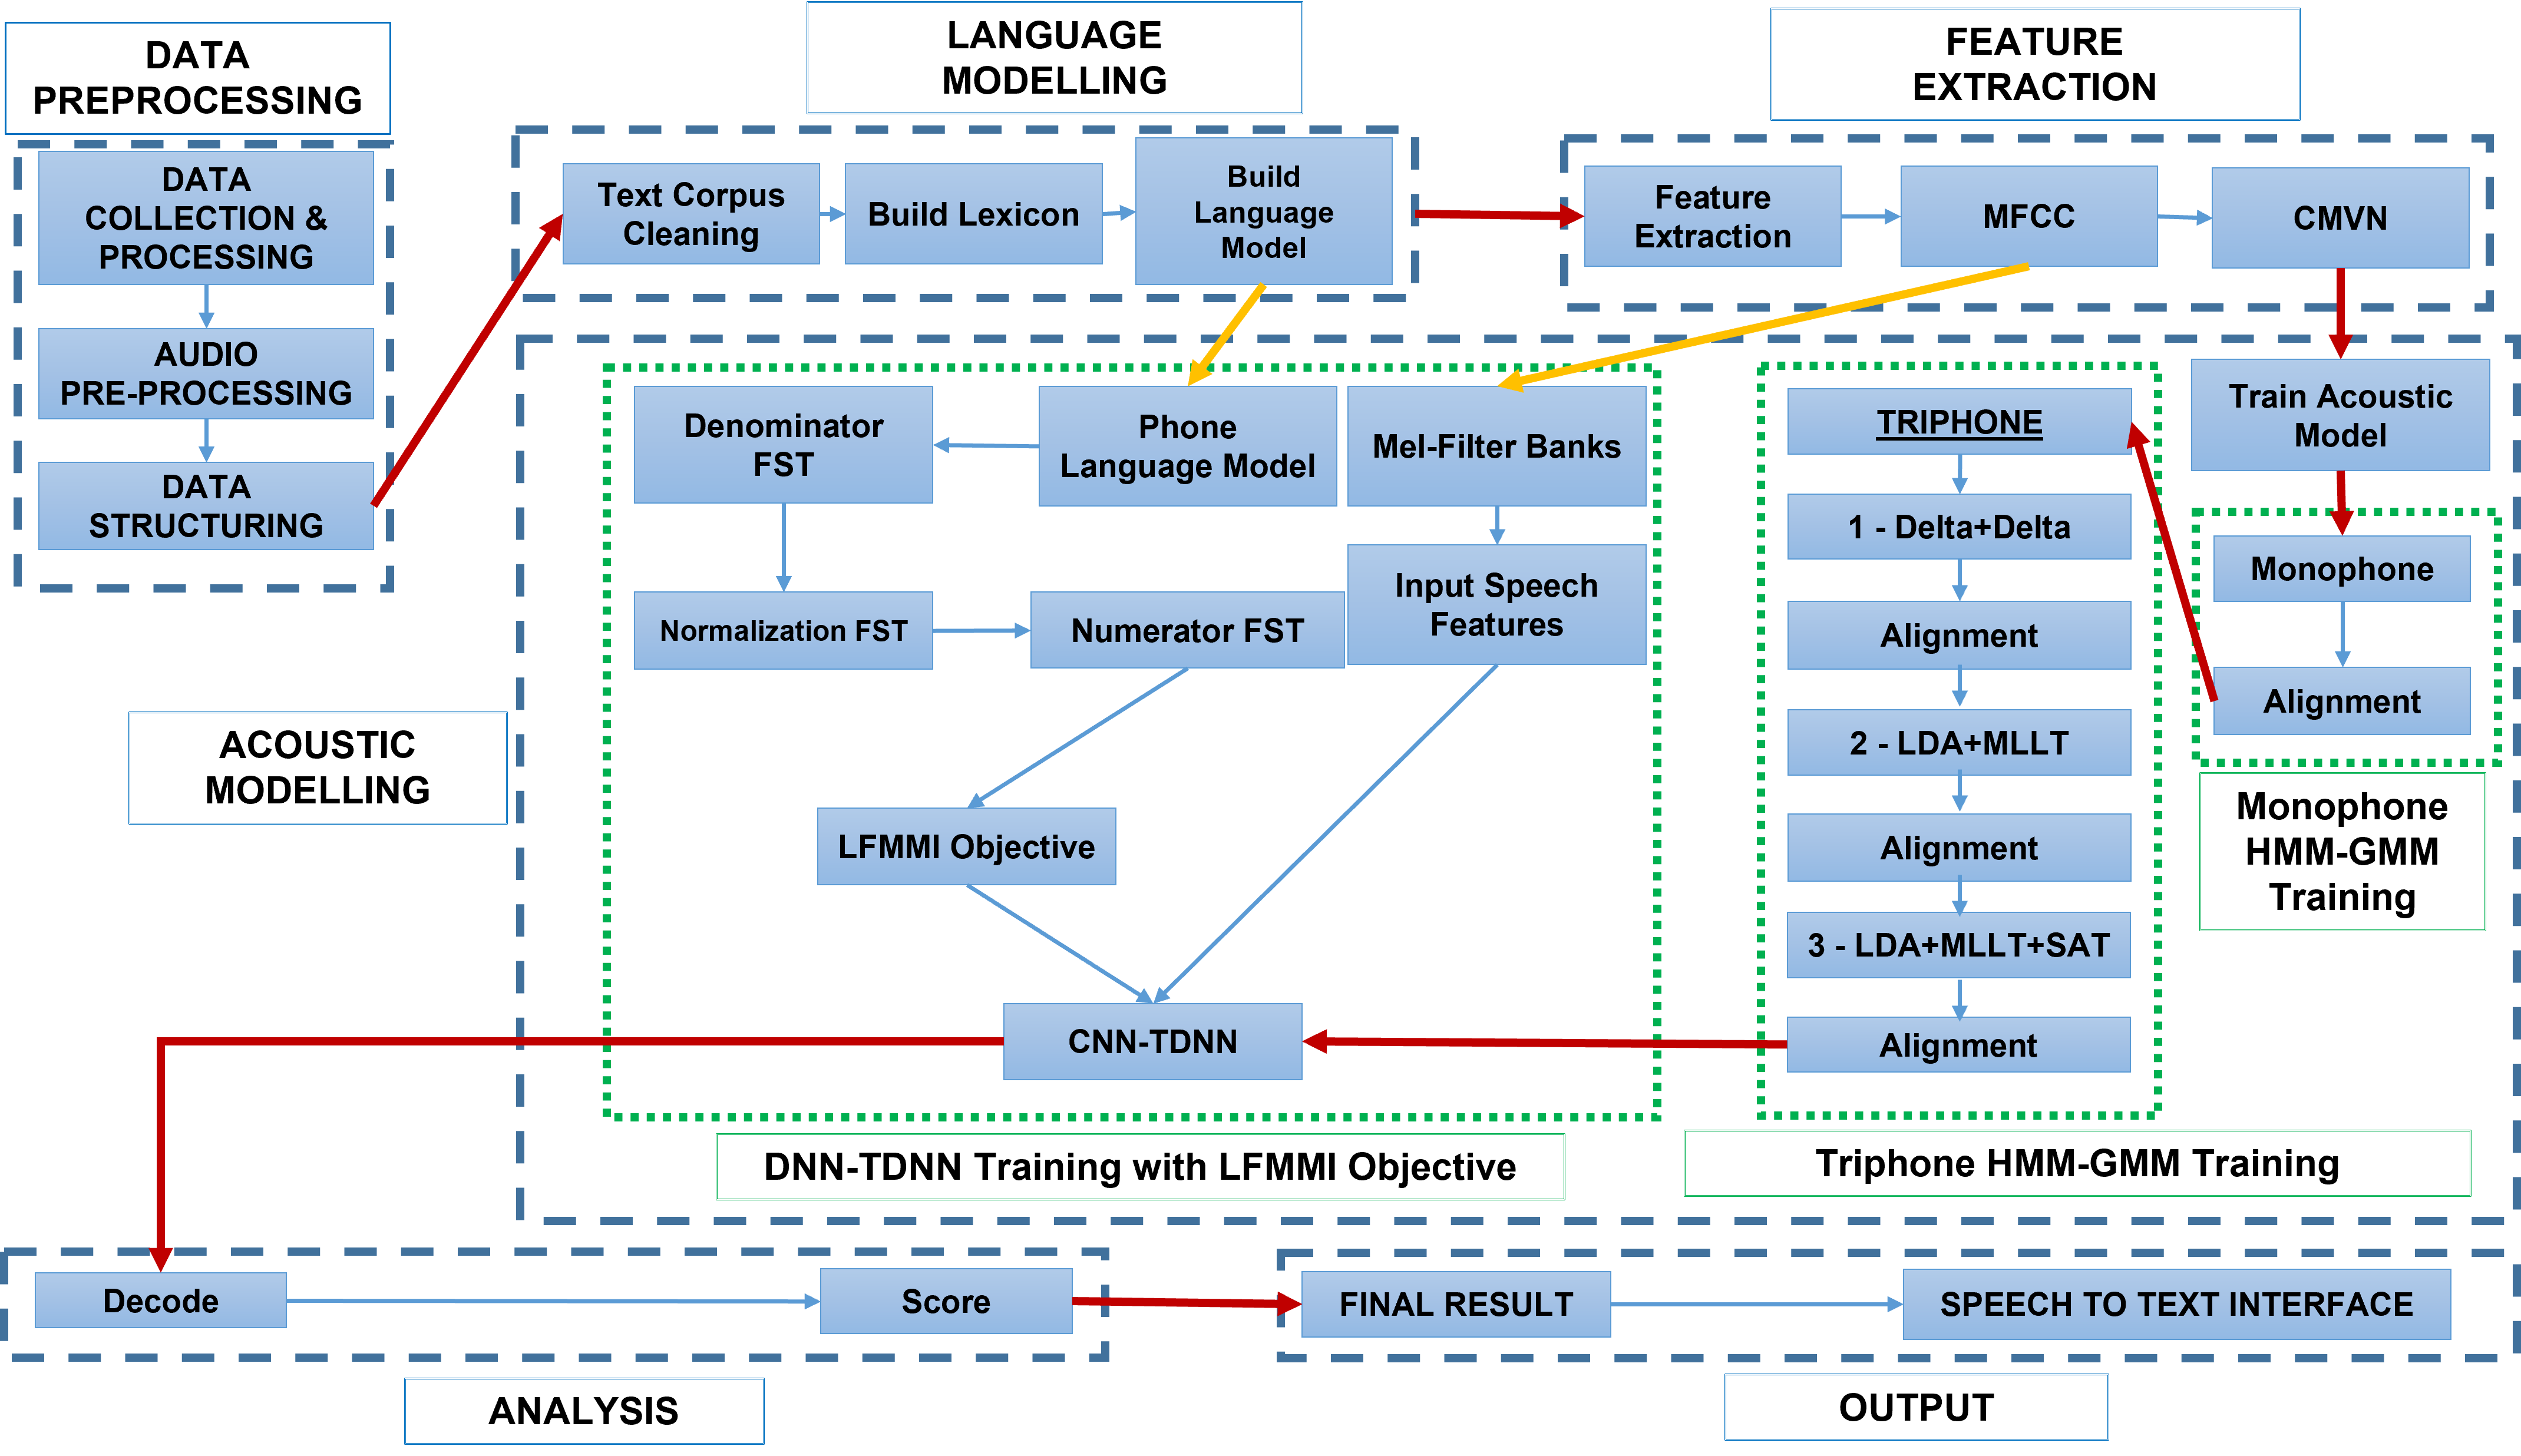
\includegraphics[width=1.5\textwidth]{img/workflow.png}
    \caption{Our Working Pipeline}
    \label{fig:working_pipeline}
\end{figure}
\end{landscape}

\newpage

%Another observation was that when compared to TDNN, CNN-TDNN tends to perform slightly better in less clean data-sets (in this case was called test-other data-set) which drew our attention towards using CNN-TDNN for training acoustic model. Many popular Deep Learning-based End to End ASR engines are available like DeepSpeech 2 \cite{amodei_deep_2015-1} but they need a massive amount of labelled data, which is not available in Urdu. Hence we decided to use CNN-TDNN for training of our Hybrid HMM-DNN ASR. Our long-term approach was to train 10 hours of data to make a strong model and use it to transcribe other audio files to build up our database to 10000 hours and then apply Deep Learning Models on the golden big data-set.

\section{Data Collection and Processing}
\label{sec:Data_preprocessing}

We had huge amount of unlabelled data available. We also had time and budget constrained. There was only one machine available in our Experimental Setup with which we had to build up the ASR. Deep Learning tends to take long time in training which means that errors will be identified after even longer time which makes the process time consuming. 

%\begin{figure}[h]
%    \centering
%    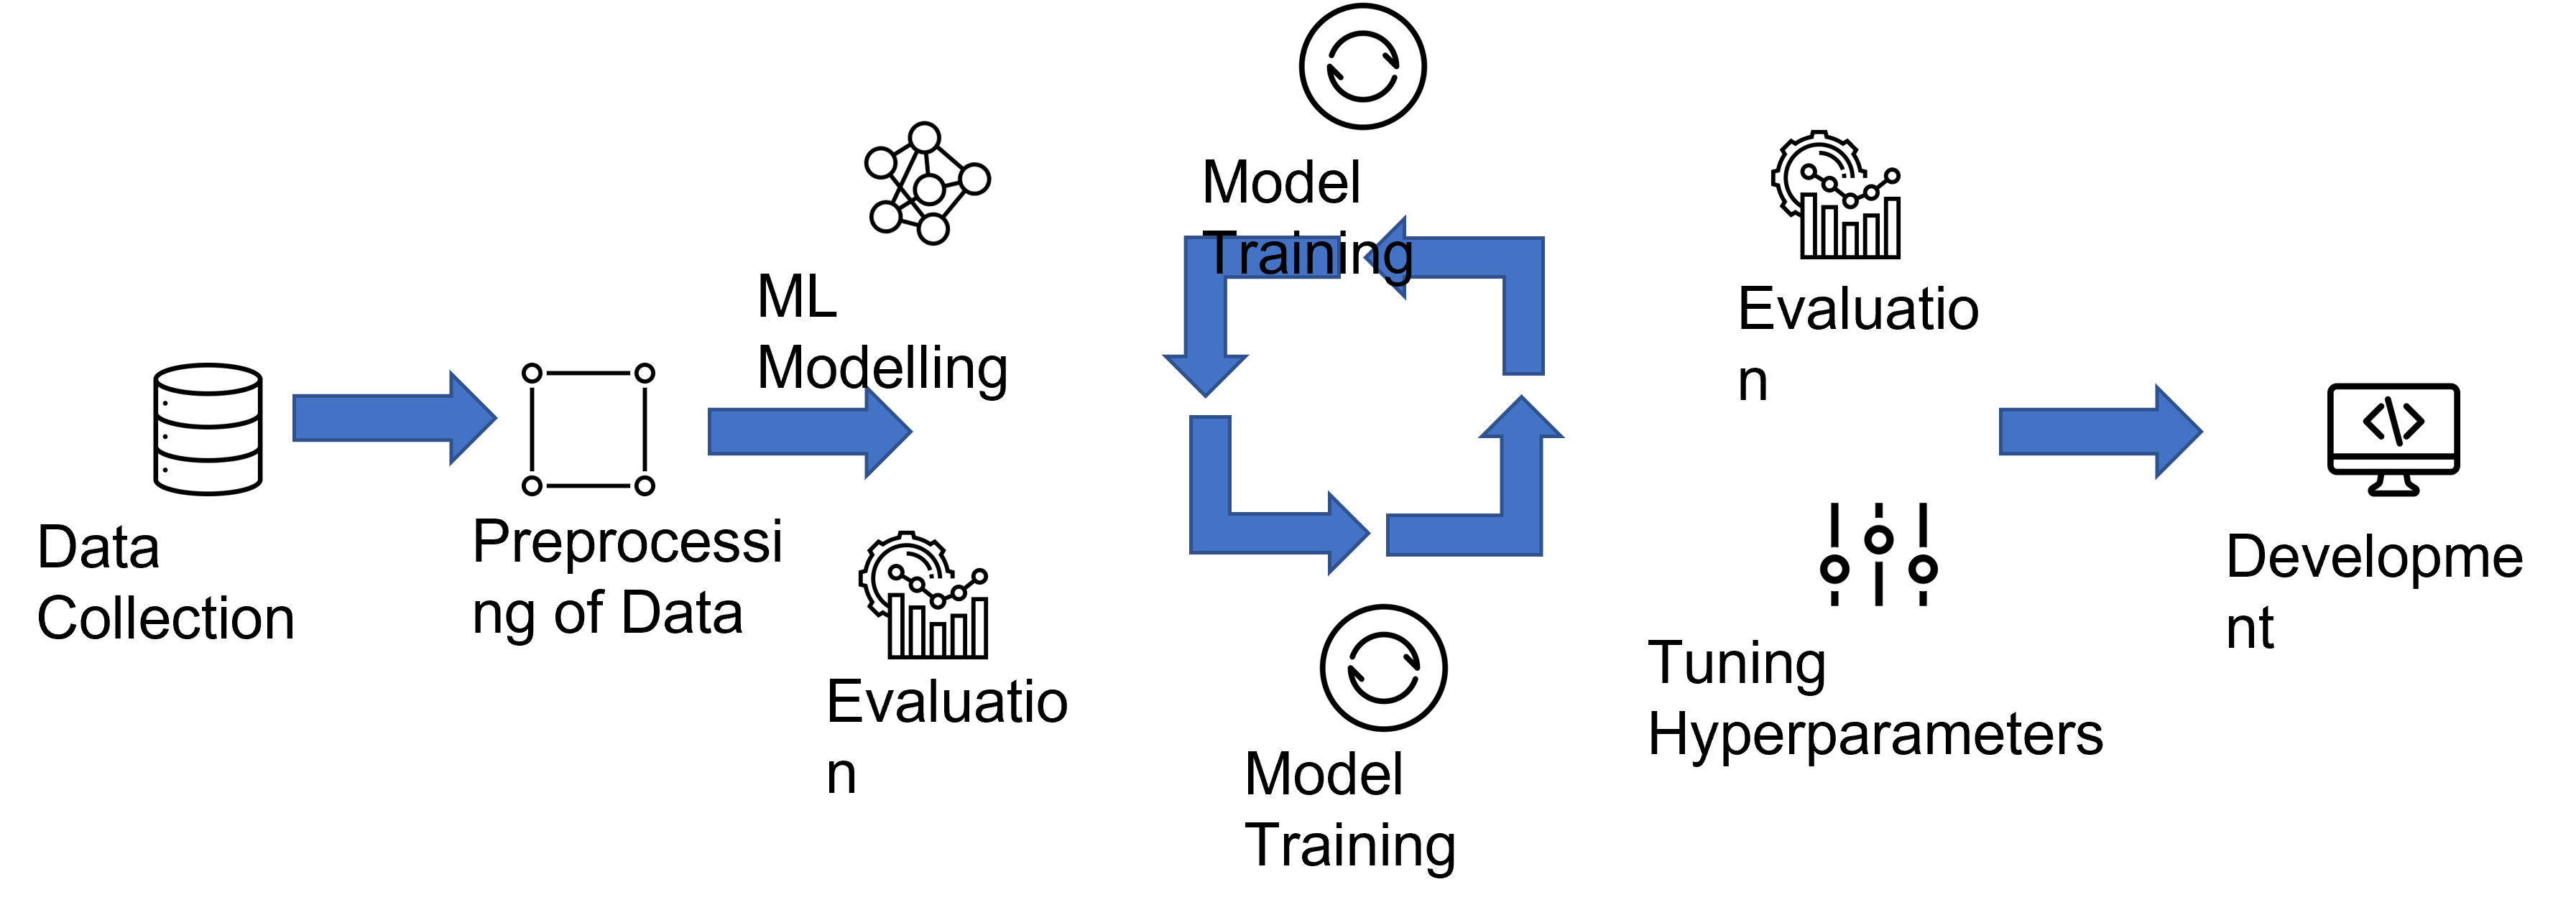
\includegraphics[width=0.9\textwidth]{img/model_centric_ml.png}
%    \caption{Model Centric Machine Learning Approach}
%    \label{fig:modelcentric-ML-approach}
%\end{figure}
%\begin{figure}[h]
%    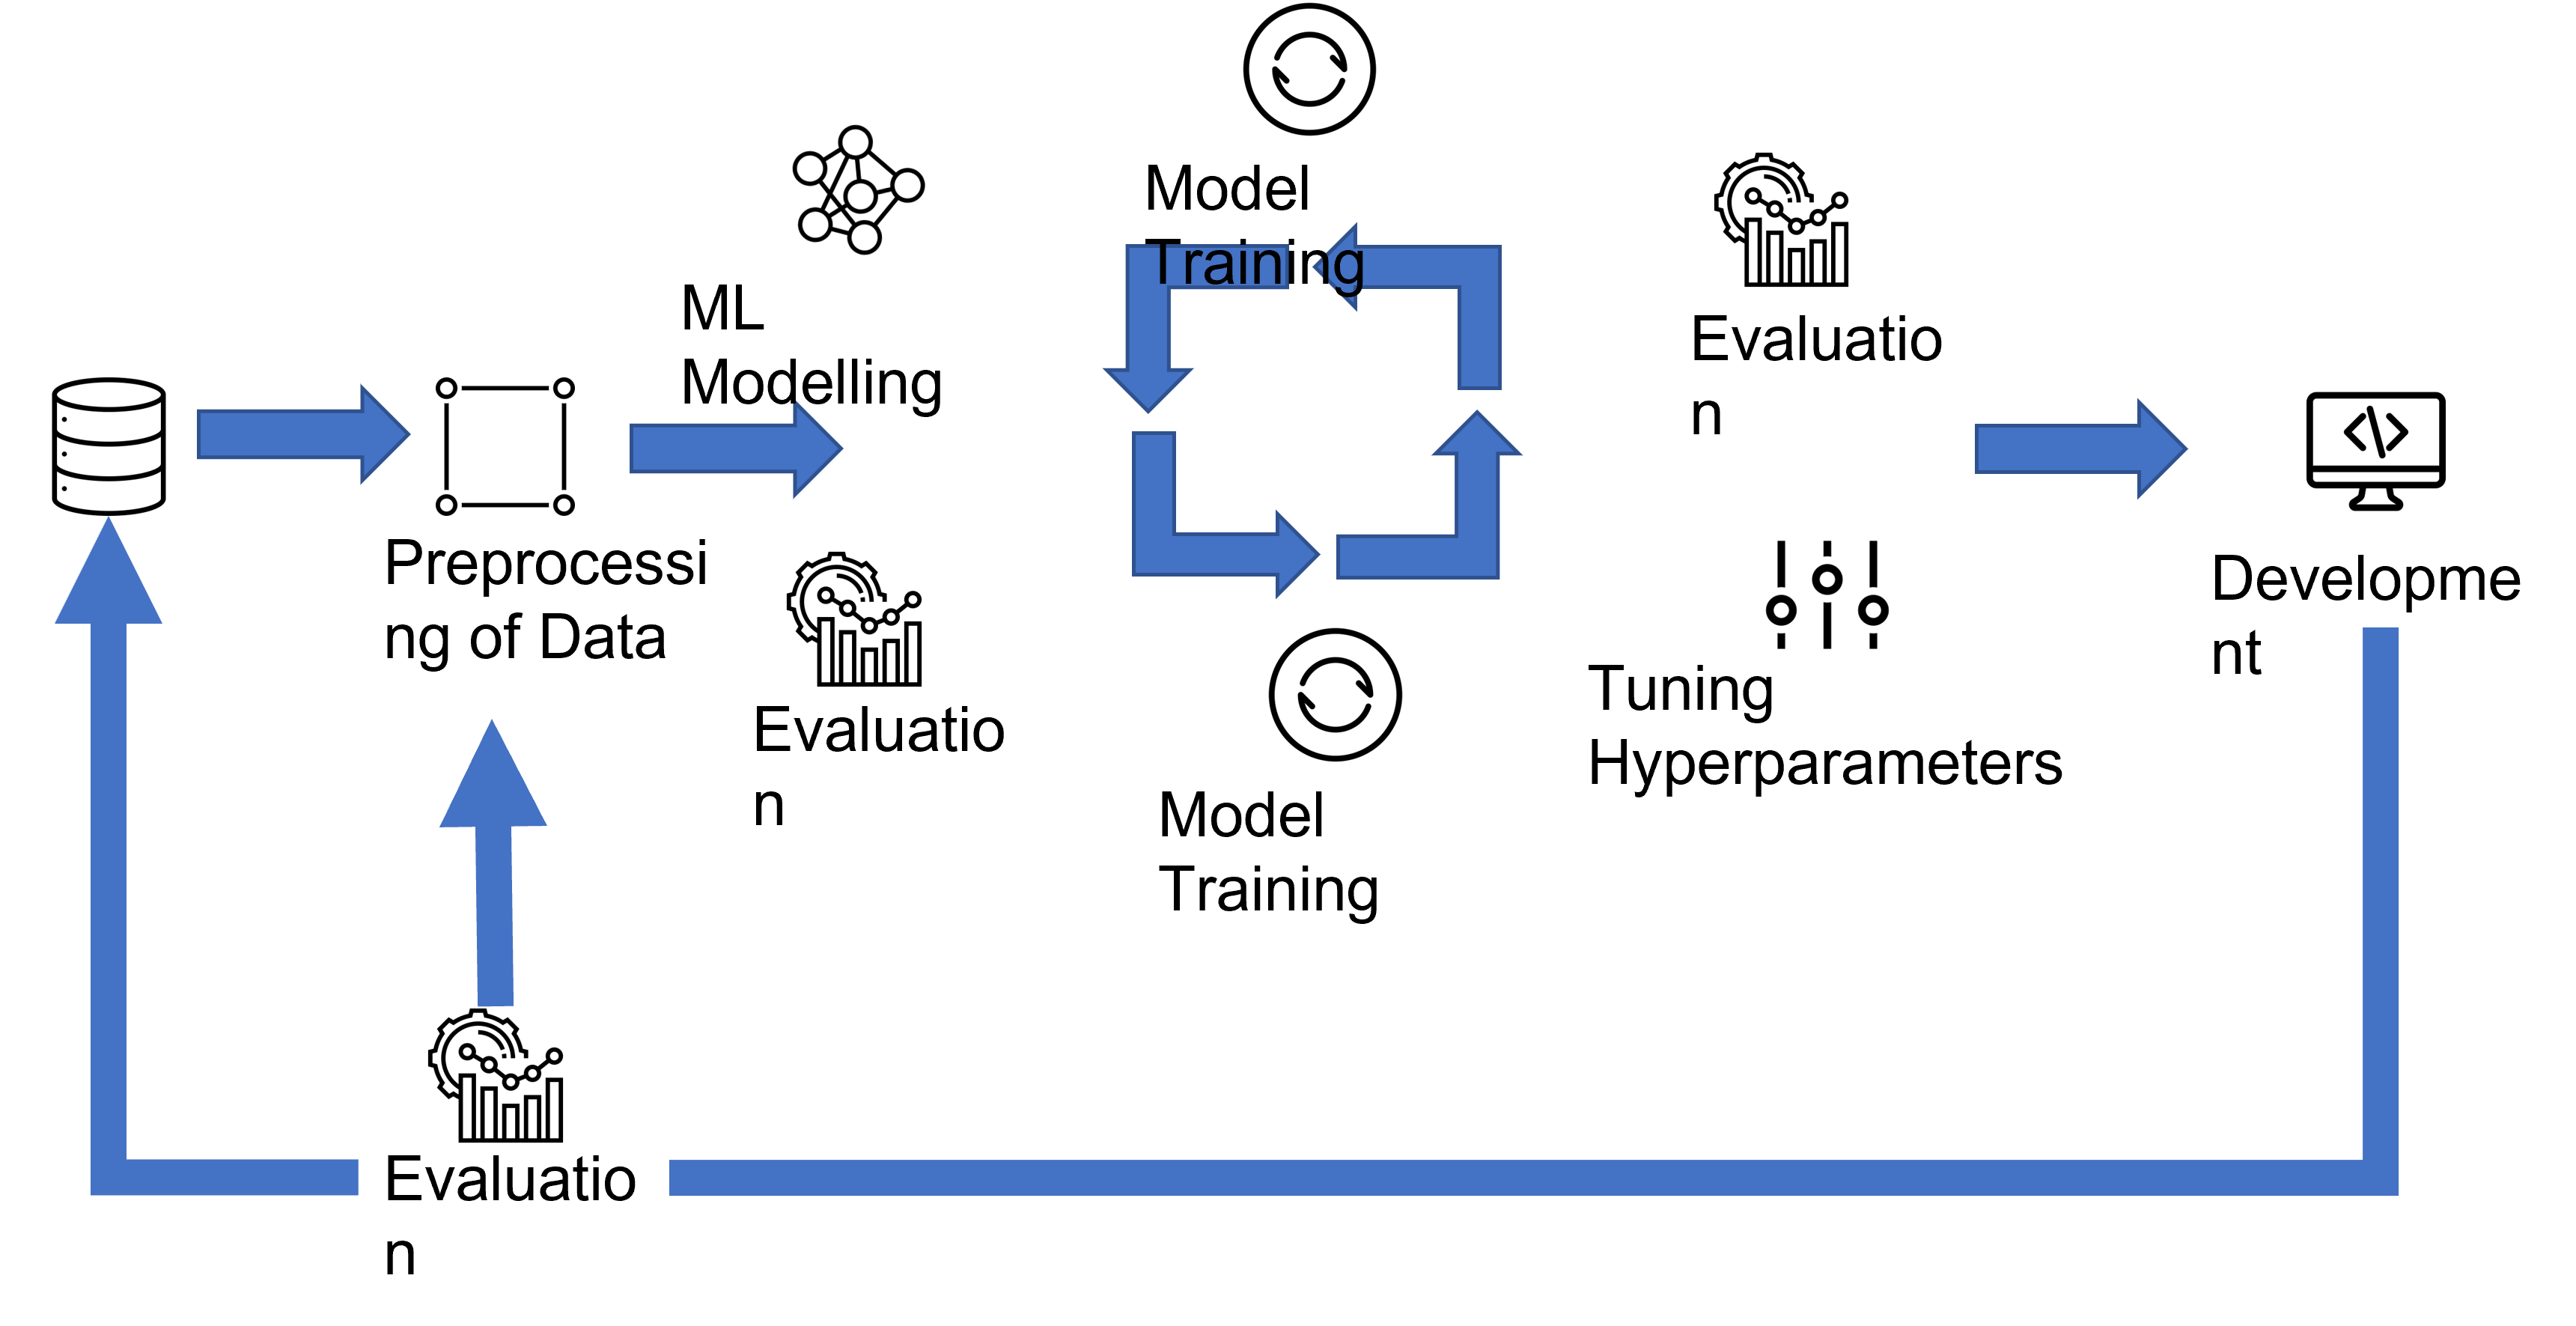
\includegraphics[width=0.9\textwidth]{img/data_centric_ml.png}
%    \caption{Data Centric Machine Learning Approach}
%    \label{fig:datacentric-ML-approach}
%\end{figure}

In this stage we focused on collection and labelling of data. The Data-Centric Approach \cite{patel_data-centric_2021} focuses on reviewing our data iteratively whenever we faced any error in the process, instead of only focusing on tweaking our model. Labelling quality of data primarily determines the overall quality of the machine model. Data is critical in AI research, and developing a strategy that prioritises obtaining high-quality data is crucial. Relevant data is not only rare and noisy, but also extremely expensive to obtain. The idea is that AI should be treated in the same way that the finest materials would be when building a house. They should be evaluated at each level rather than just once.

The common question is how much data is enough to build a quality model? We are often told more data means more accurate model. However, in any given scenario, Quality trumps quantity and same is what we tried to ensure. A data-set with millions of rows with a lot of noisy observations can lead to an obscured learning process, while a smaller data-set with good quality labels tends to give much better results. Eventually we would want a huge dataset that is accurately annotated on which we can make use of End to End ASR training.

\subsection{Data Sources} 
\label{sub:datasources}
We had a mix of structured and unstructured data, with varying duration (1-20 seconds), available from following sources:
\begin{itemize}
    \item D1 - PRUS \cite{zia_pronouncur_2018} 708 sentences data-set taken from \cite{qureshi_urdu_2021}.
    \item D2 - Sehar’s data-sets \cite{sehar_gul_detecting_2020}
    \item D3 - 250 Isolated words data-set \cite{asadullah_automatic_2016} \cite{noauthor_urdu_nodate}. 
    \item D4 - English and Urdu Alphabet spoken audio data which we collected and labelled ourselves.
        \item D5 - Call center unlabelled audio.
\end{itemize}

\subsection{Audio Pre-Processing}

The sampling rates of audio was largely mixed i.e. some had 8KHz and others had 16KHz frequency. We chose a higher sampling rate of 16000 Hz to have more information of speech signal is saved in the noisy or telephonic data. Generally, for ASR training, it is preferred \cite{noauthor_kaldi_nodate} that audio files with mono channel with 8kHz or 16kHz sampling frequency are used \cite{noauthor_why_nodate}. 

We required mono audio in wav format for training \cite{noauthor_kaldi_nodate} \cite{noauthor_why_nodate}. Most of our data was available in mono and for conversion we our customized script using SoX and ffmpeg \cite{noauthor_sox_nodate}.Wav files, unlike mp3, are raw audio and have no compression applied to them which means there is no loss of information in the audio file.

\begin{figure}[htb]
    \centering
    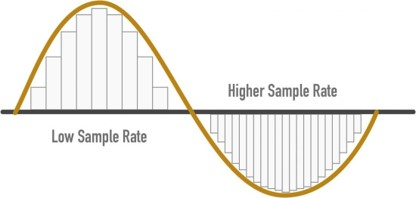
\includegraphics[scale=0.8]{img/samplingrate.jpg}
    \caption{High Sampling Rate vs Low Sampling Rate}
    \label{fig:sampling-rate-high-low}
\end{figure}

Instead of removing noise to maintain speech, we made sure that each utterance had a clean and a noisy counterpart. The ASR would then know for instance how a clean utterance of the word "salaam" sounds like and how "salaam" sounds in noisy environment. Hence we decided to use a higher sampling rate so that more information is retained in the audio. 
%https://en.wikipedia.org/wiki/Sample-rate_conversion

\subsection{Data Structuring}
Our unstructured data-set was the major challenge. We had more than 500 hours of unstructured audios of Call center but we could not spend all the time making We analyzed the scenario of the Call Center and found that the calls were mostly Verification calls which meant primarily we needed good recognition of digits and alphabets in English and Urdu. The normal conversational words were greetings and goodbyes which were standard sentences.

\begin{itemize}
    \item We selected some calls and split them word/sentence/speaker-wise and transcribed them to be included as part of the training set. 5 splits were made speaker wise with utterances for speakers being 348, 8, 7, 55 and 12 clips.
    \item For test 38 utterances were set aside separate to the structured data to judge the results separately. These clips were taken at random, containing out-of-vocabulary words, overlapping speech, distortion and low volume at times, just like in real-life scenario.
    \textit{Note: On average utterances in all cases were 1-20 seconds, covering either single words, multiple words, or up to 3 sentences.} 
\end{itemize}

%For comparison these were also run through google speech recognition API (offline), vocalmatic (online) simonsaysai (online), and dictation.io. The results were 99.9\% error
 
The total audio length for training was 6hours 47minutes and testing was 3h17m. The utterances which sliced from calls were given 0.5-1 second silence in start and end to ensure that there are is no abruptness in the clips, making it easier for ASR to process and align. 

We divided our data into two types; structured and unstructured. Structured data-sets had labeling and transcriptions available whereas the unstructured data-set had no labeling and transcriptions available. 

With regard to the structured data-set the data organization was as follows:
\begin{enumerate}
    \item \textbf{D1:} PRUS \cite{zia_pronouncur_2018} data set (along with Zoraiz Qureshi) 
    \begin{itemize}
        \item Total 7 speakers, 708 sentence-utterances per speaker
        \item Train set = 4 and Test set = 3
    \end{itemize}
    \item \textbf{D2:} Sehar Data-set \cite{sehar_gul_detecting_2020} 
    \begin{itemize}
        \item 100 Sentence-utterances (Malicious), 3 x speakers; 2 x Train and 1 x Test
        \item 86 Sentence-utterances, 7 x speakers; 5 x Train 2 x Test
        \item 5 Word-utterances, 13 x speakers; 10 x Train, 2 x Test
    \end{itemize}
    \item \textbf{D3:} 250-word data set from Asadullah \cite{asadullah_automatic_2016} \cite{noauthor_urdu_nodate} which was also used by Sehar. This had the transcription in Urdu so we had to manually do the transcription in Roman Urdu since that was our chosen mode of writing to avoid spending time building different language models and blending them.    \begin{itemize}
        \item 10 Speakers;
        \item 8 x Train, 2 x Test
    \end{itemize}
    \item \textbf{D4:} English and Urdu Alphabet data which we collected ourselves  
    \begin{itemize}
        \item 11 x Speakers in the Train set. Number of Utterances by each speaker was 28, 102, 206, 60, 28, 26, 37, 135, 256, 185 and 116 clips.
        \item 4 x Speakers in the Test set. Number of Utterances by each speaker was 52, 53, 44 and 55 clips 
    \end{itemize}
    \item \textbf{D5:} Telephonic Data-set samples  
    \begin{itemize}
        \item Training - 5 x speakers and Utterances= 348, 8, 7, 55, 12 clips.
        \item For validation 38 utterances from 2 Speakers
    \end{itemize}
\end{enumerate}

\section{Language Model}
\label{sec:our_lang_modelling}

LM finds the probabilities of words succeeding or preceding a specific word in a given sequence i.e. estimation of likelihood of a word-sequence $W = w_{1},...,w_{n}$ forming a valid sentence, thereby reducing the search radius of the decoders. It can be used to make decisions when the acoustic model output consists of a set of phonemes which can form various alternative sentences. Although these alternatives may be very acoustically similar, the LM selects the one that makes the most sense. LMs are usually formatted in ARPA form which are converted into Finite State Transducers in ASR engines like Kaldi.

\begin{figure}[htb]
    \centering
    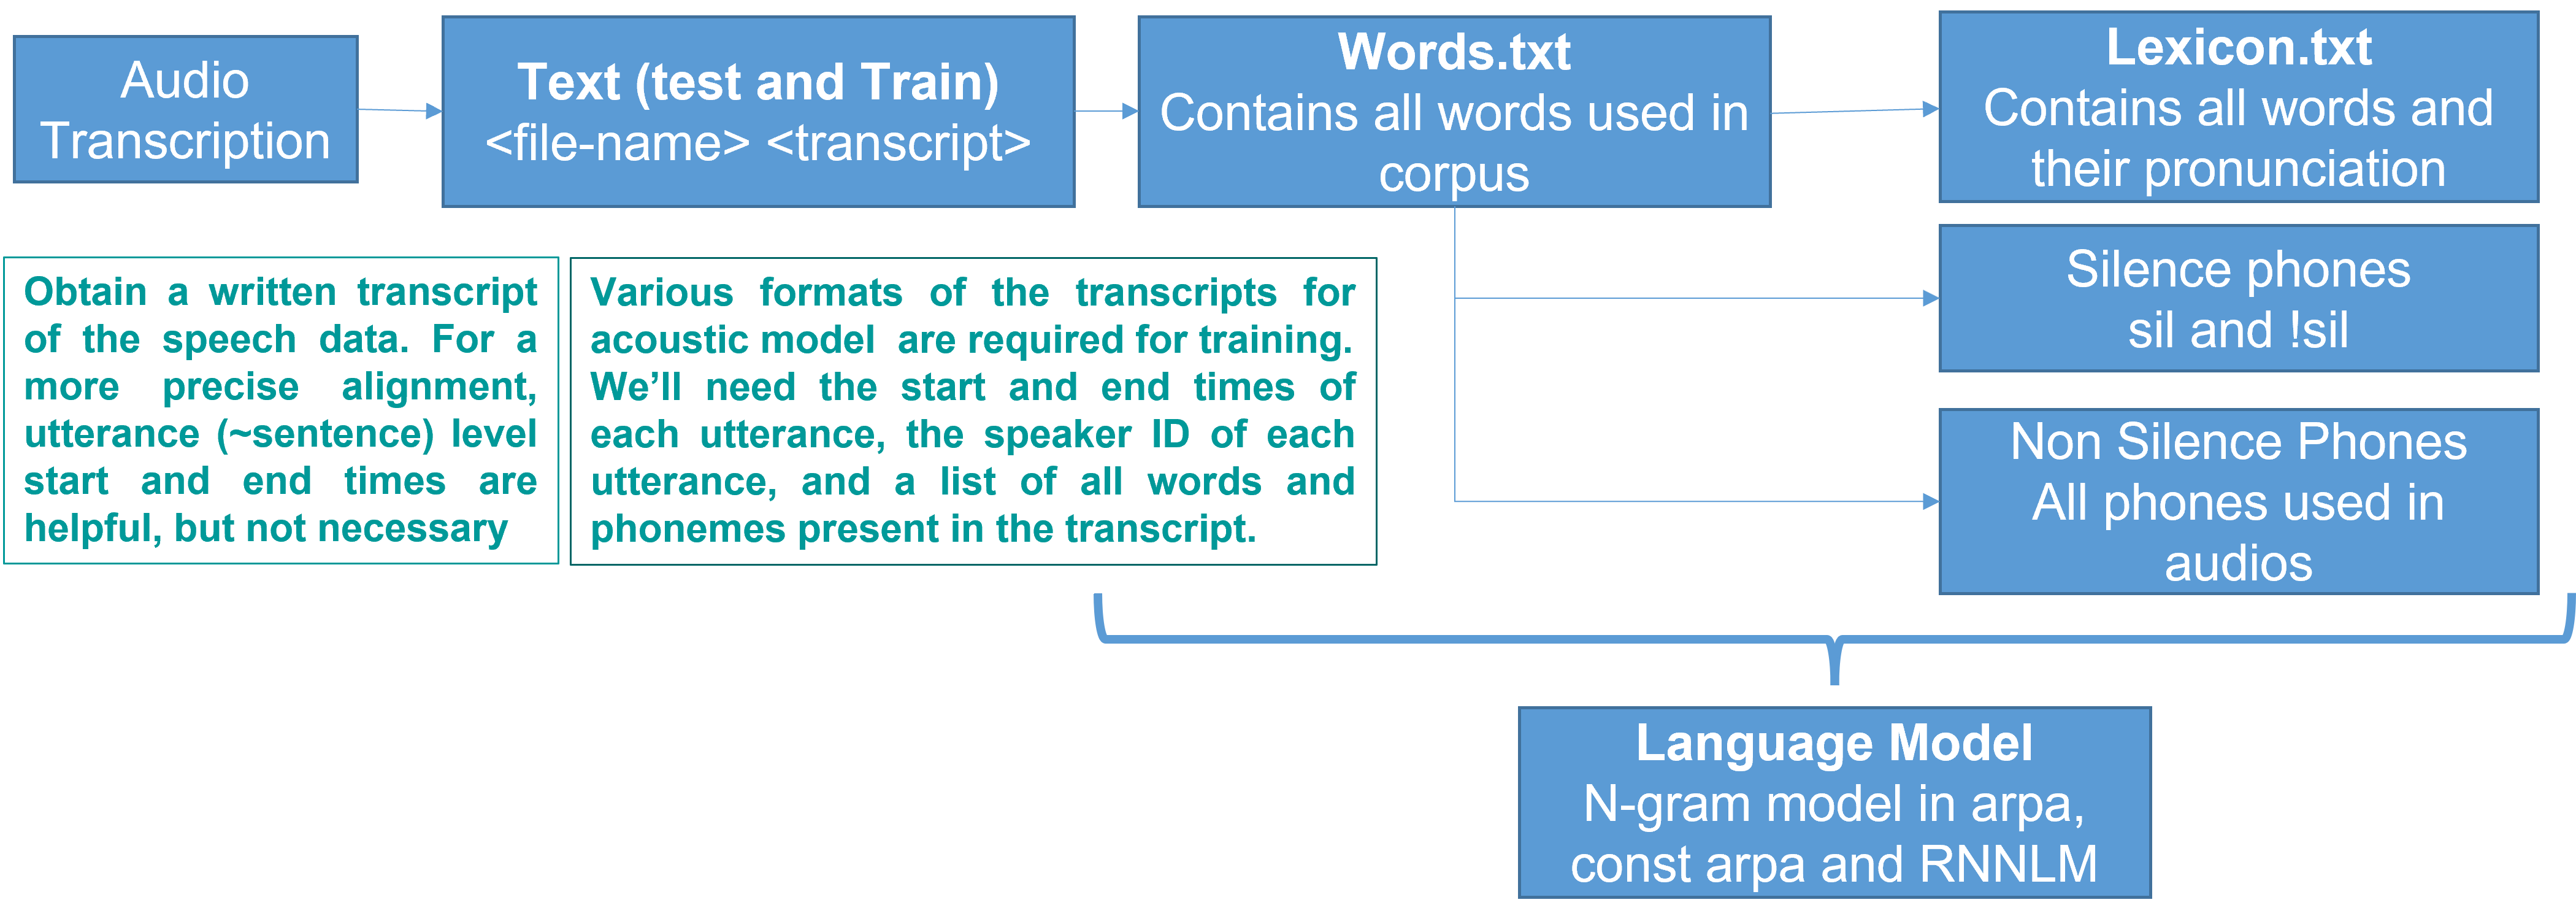
\includegraphics[width=0.95\textwidth]{img/LM.png}
    \caption{Language Model Preparation process}
    \label{fig:lang-model1}
\end{figure}

\subsection{Text Corpus Cleaning}

To prepare LM we combined the transcripts of test and train files in their respective files called \textit{"text"} which contains file-names in one column and their transcripts on the other column. We filtered the corpus and took out all unique words in the text using \textit{cut, sed, uniq and sort} in Linux and saved it as \textit{"words.txt"} \cite{chodroff_corpus_2018}. 

\subsection{Building Lexicon}
There were 7333 words, 137 phones, and 75 non-silence phones in the lexicon, each phoneme represented by a unique combination of symbols and letters. A silence phoneme, 'sil' is added to the 137 phonemes to represent the silence between hyphenated words or the beginning or end of a sentence. The mapping from speaker to utterance was done in spk2utt and utt2spk files.

The English script was used as symbol representations to create a dictionary that shows how words are mapped to phoneme sequences. Word to phoneme dictionary was prepared with help of lextool by CMU \cite{cmu_cmu_nodate} and saved it as \textit{"lexicon.txt"}. Using pronunciation probabilities, multiple pronunciations of the same words were also included.  

\subsection{Building Language Model}

We used SRILM \cite{andreas_stolcke_srilm_2002} for language modelling and building grapheme to phoneme (g2p) sequence-to-sequence model for phonetic mappings of generated lexicon. It was done in local environment to avoid issues with colab \cite{naeem_subspace_2020}. 

There are various types of language modelling based on the number of phonemes considered at once. Assume we have a k-length sequence. Let $P(w_{1}, w_{2}, w_{3},..., w_{k})$ denote the probabilities assigned to the entire sequence by LM. We used a traditional n-gram model using SRILM \cite{andreas_stolcke_srilm_2002}. For an n-gram model, the probability of any word sequence $P(w_{1}, w_{2}, w_{3},..., w_{k})$ is then given as:

\begin{equation}
P(w_{1},w_{2}...,w_{k}) = \prod\nolimits_{i = 1}^{k} a_{i} P(w_{i} | w_{1},...,w_{i-1})
\end{equation}

\section{Feature Extraction and Acoustic Modelling}
\label{sec:feature-extraction-and-AM}
This part computes features from speech wave-form containing elevant information about the linguistic content of the speech while ignoring background noise, emotions etc. The extracted features represent the phones within the words, while other signal-degrading elements such as channel characteristics and background noise are suppressed. MFCC and Perceptual Linear Prediction Coefficients are two popular feature extraction methods (PLP) \cite{backstrom_introduction_2022}. We used the MFCC feature extraction method in our work.  

\begin{figure}[h]
    \centering
    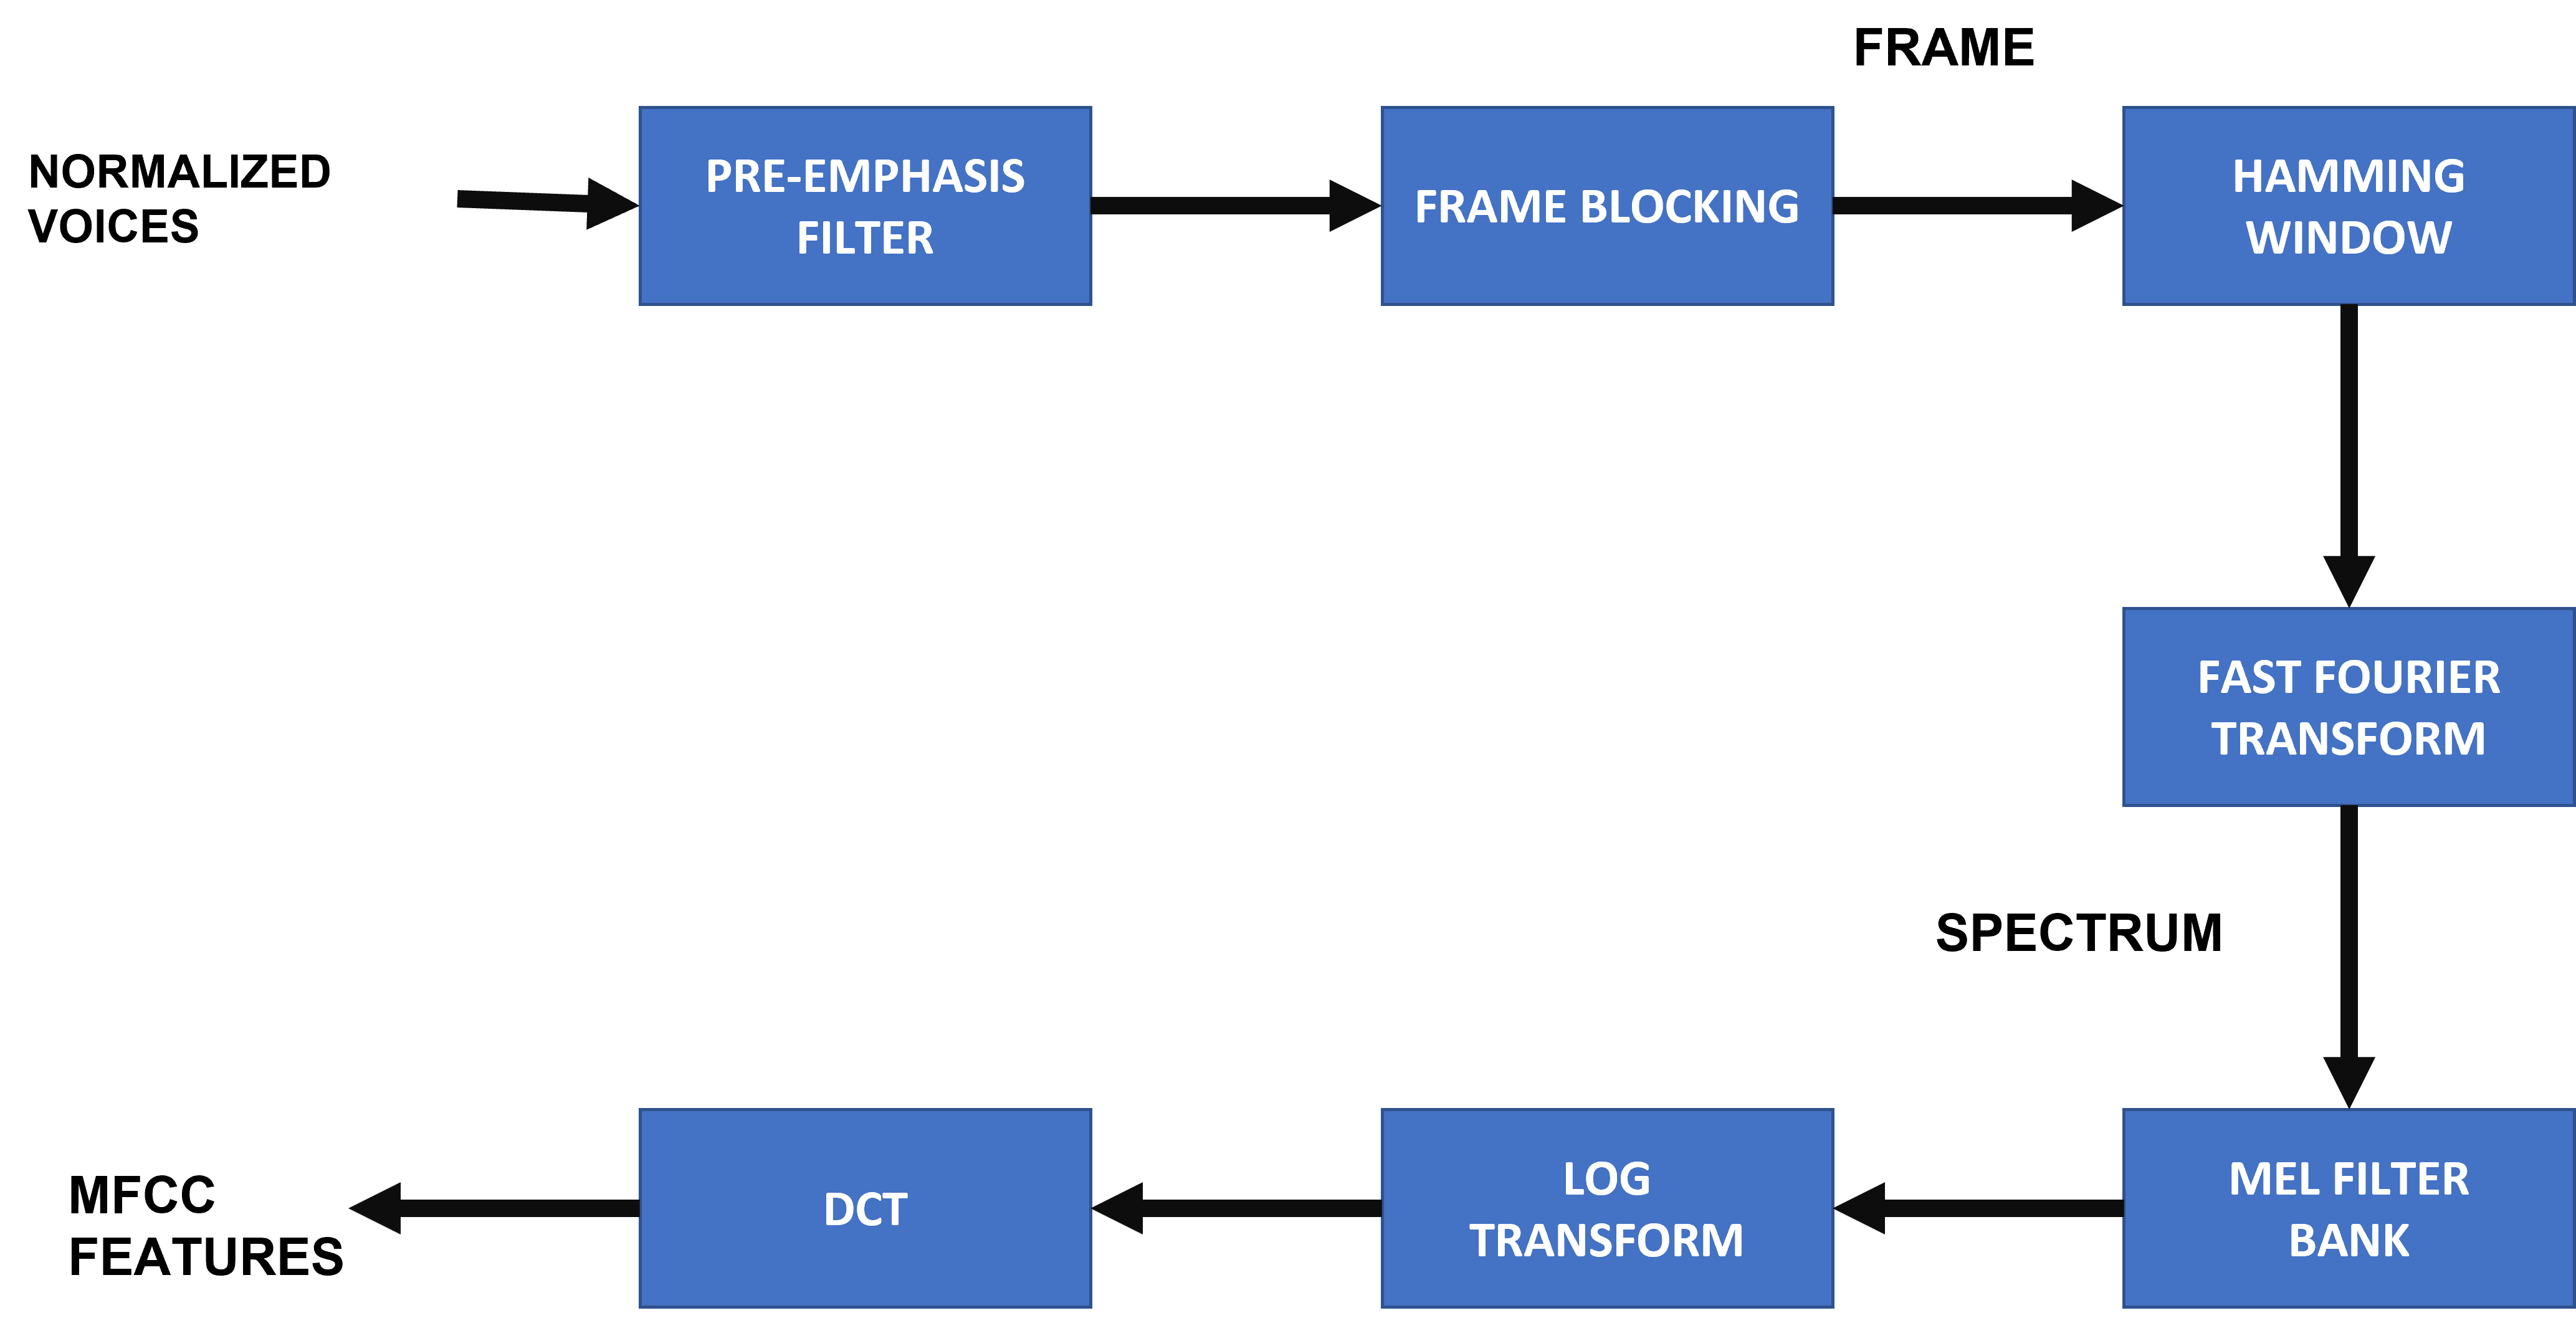
\includegraphics[width=0.8\textwidth]{img/feature extraction.png}
    \caption{Feature Extraction Process}
    \label{fig:Feature-extraction}
\end{figure}

\subsection{MFCC}
\label{sub:MFCC-trg}

The reason MFCC is still extensively used \cite{noauthor_kaldi_nodate} is because they are more easily compressible, being de-correlated; we dump them to disk with compression to 1 byte per coefficient. But we dump all the coefficients, so it’s equivalent to filter-banks times a full-rank matrix without any information loss \cite{raj_note_nodate}. 

MFCCs has a historical momentum and everyone is familiar with it. Hence there is no requirement switch to another model from a familiar one without a very strong reason. If the machine learning algorithm is susceptible to correlated input we use MFCC, a common use case of which are HMM-GMM statistical ASR models. We use Mel-scaled filter banks if the machine learning algorithm is not susceptible to highly correlated input like Neural Networks. 

We extracted 40 MFCCs with  window size of 25ms and 10ms shift, from our training data \cite{naeem_subspace_2020}. The MFCC extraction process begins by conversion of Analogue signals to Digital so that computers can understand them. The next step, Pre-emphasis boosts the energy present in the higher frequencies to counter the spectral tilt issue which is that lower frequencies have more energy. Energy in the higher frequencies are enhanced for easy detection of third formant or F3 i.e. one of the three formants in a phoneme. 

The next step is windowing which is the process of slicing an audio waveform into small overlapping frames because each frame represents a single phoneme which is why we must carefully choose the window length. The entire waveform is divided into 20-40 ms segments. The assumption is that the signal is statistically stationary in this short segment, so features can be assumed to be constant inside this window \cite{raj_note_nodate}. 

Windows overlap as they are 25 ms long and spaced 10 ms apart. In one window, approximately 400 samples are reduced to 13 Cepstral coefficients. The feature is enhanced with additional 13 delta and 13 delta-delta coefficients making a total of 39 Features. Using Hamming Window, this method smooths down the sudden edges in each frame. DFT is then applied to transfer information from the time to the frequency domain. 

After this, a set of triangular band pass filters called Mel filter are applied to the waveform after squaring the DFT output which converts information to the power spectrum. The power spectrum (or estimate of the spectral density of a signal called periodogram) is computed to recognise the frequencies present in this short segment which is accomplished through the use of discrete-time Fourier transforms.  

\subsection{Cepstral Mean and Variance Normalization}
\label{sub:CMVN}
Cepstral calculation as shown in \ref{fig:cepstral} isolates the source from the filter. Pitch information is removed by MFCC features as it is not required in the Speech To Text scenario. The log spectrum contains information about the phone and the pitch. The formants that distinguish phones are identified by the peaks in the spectrum. The IFT can be applied to separate the pitch information from the formants. All that is left to do is take the first 12 independent cepstral values.

\begin{figure}[htb]
    \centering
    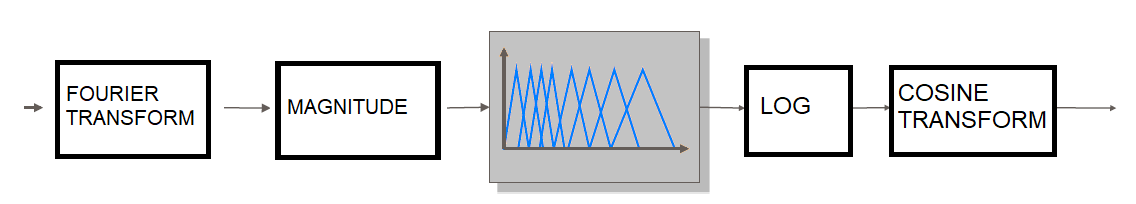
\includegraphics[width=0.8\textwidth]{img/cepstral.png}
    \caption{Cepstral Calculation}
    \label{fig:cepstral}
\end{figure}

Cepstral mean and variance normalisation (CMVN) is a popular noise compensation technique used in a variety of speech applications. It is a computationally efficient noise robust speech recognition normalisation technique. By transforming them to zero mean and unit variance, CMVN eliminates the mismatch between training and test utterances. CMVN performance is known to degrade for short utterances due to a lack of data for parameter estimation and a loss of discriminable information because all utterances are forced to have a zero mean and unit variance.

Cepstral Mean and Variance Normalization techniques (\ref{sub:CMVN}) are most effective for long utterances. Histogram Equalization (HEQ) outperforms CMVN and Cepstral Mean Normalization (CMN) because it matches all moments of the training and test utterances. CMVN matches only the mean and variance while CMN matches only the mean. 

CMVN and HEQ perform worse for short utterances due to a lack of data for parameter estimation. Normalization removes some useful information by forcing all utterances to have the same first and second-order statistics, i.e. zero mean and unit variance \cite{joshi_modified_2016}.

\section{Acoustic Modelling}
\label{sec:training_the_model}

%Kaldi provides various tools to train Acoustic models. We chose to train a Hybrid HMM-DNN model (\ref{sec:hybrid HMM-DNN}) because:
%\begin{itemize}
%    \item We had very limited labeled data. Hence, going completely for Deep %Learning is of no good use.
%    \item Statistical approach may have limitations as discussed earlier but with less data, it works well.
%    \item Our approach was to train 10 hours of data to make a strong model and use it to transcribe other audio files to build up our database and then apply DNN.
%\end{itemize}

In this section we will discuss our Acoustic Model training. Acoustic models are statistical representations of the acoustic information in a phoneme which convert the audio features we created into a sequence of context-dependent phonemes and are required for both automatic speech recognition and forced alignment. 

Various acoustic models such as Mono-phone, Tri-phone, and Chain CNN-TDNN are used to compute the Word Error Rates to validate the ASR system. The dictionary contained 7333 words and 137 phonemes (75 non silence phonemes) based on our training corpus.

Time markings on the phonemes are required for alignment. Hence, the system divides each audio file into equal alignments during alignment, with each division mapped to a different phoneme symbol in the sequence. Each model further refines the alignments using various training techniques before passing them on to the next stage, which is then used for recognition.

We first trained the GMM-HMM model with our training data-set before we can train the DNN-HMM model \cite{li_hybrid_2013}. HMM-DNN acoustic modeling consists of the following steps:
\begin{enumerate}
    \item Mono-phone Training (HMM-GMM).
    \item Tri-phone Training (HMM-GMM) with: 
    \begin{enumerate}[label=\alph*]
        \item Delta features
        \item Delta and delta-delta features
        \item Linear Discriminative Analysis (LDA)
        \item Maximum Likelihood Linear Transform (MLLT)
        \item Speaker adapted training (SAT), i.e. training on feature space maximum likelihood linear regression (fMLLR) adapted features
    \end{enumerate}
    \item HMM-DNN model training using LF-MMI and CNN-TDNN \cite{ghahremani_acoustic_2016}.
\end{enumerate} 

\begin{figure}[h]
    \centering
    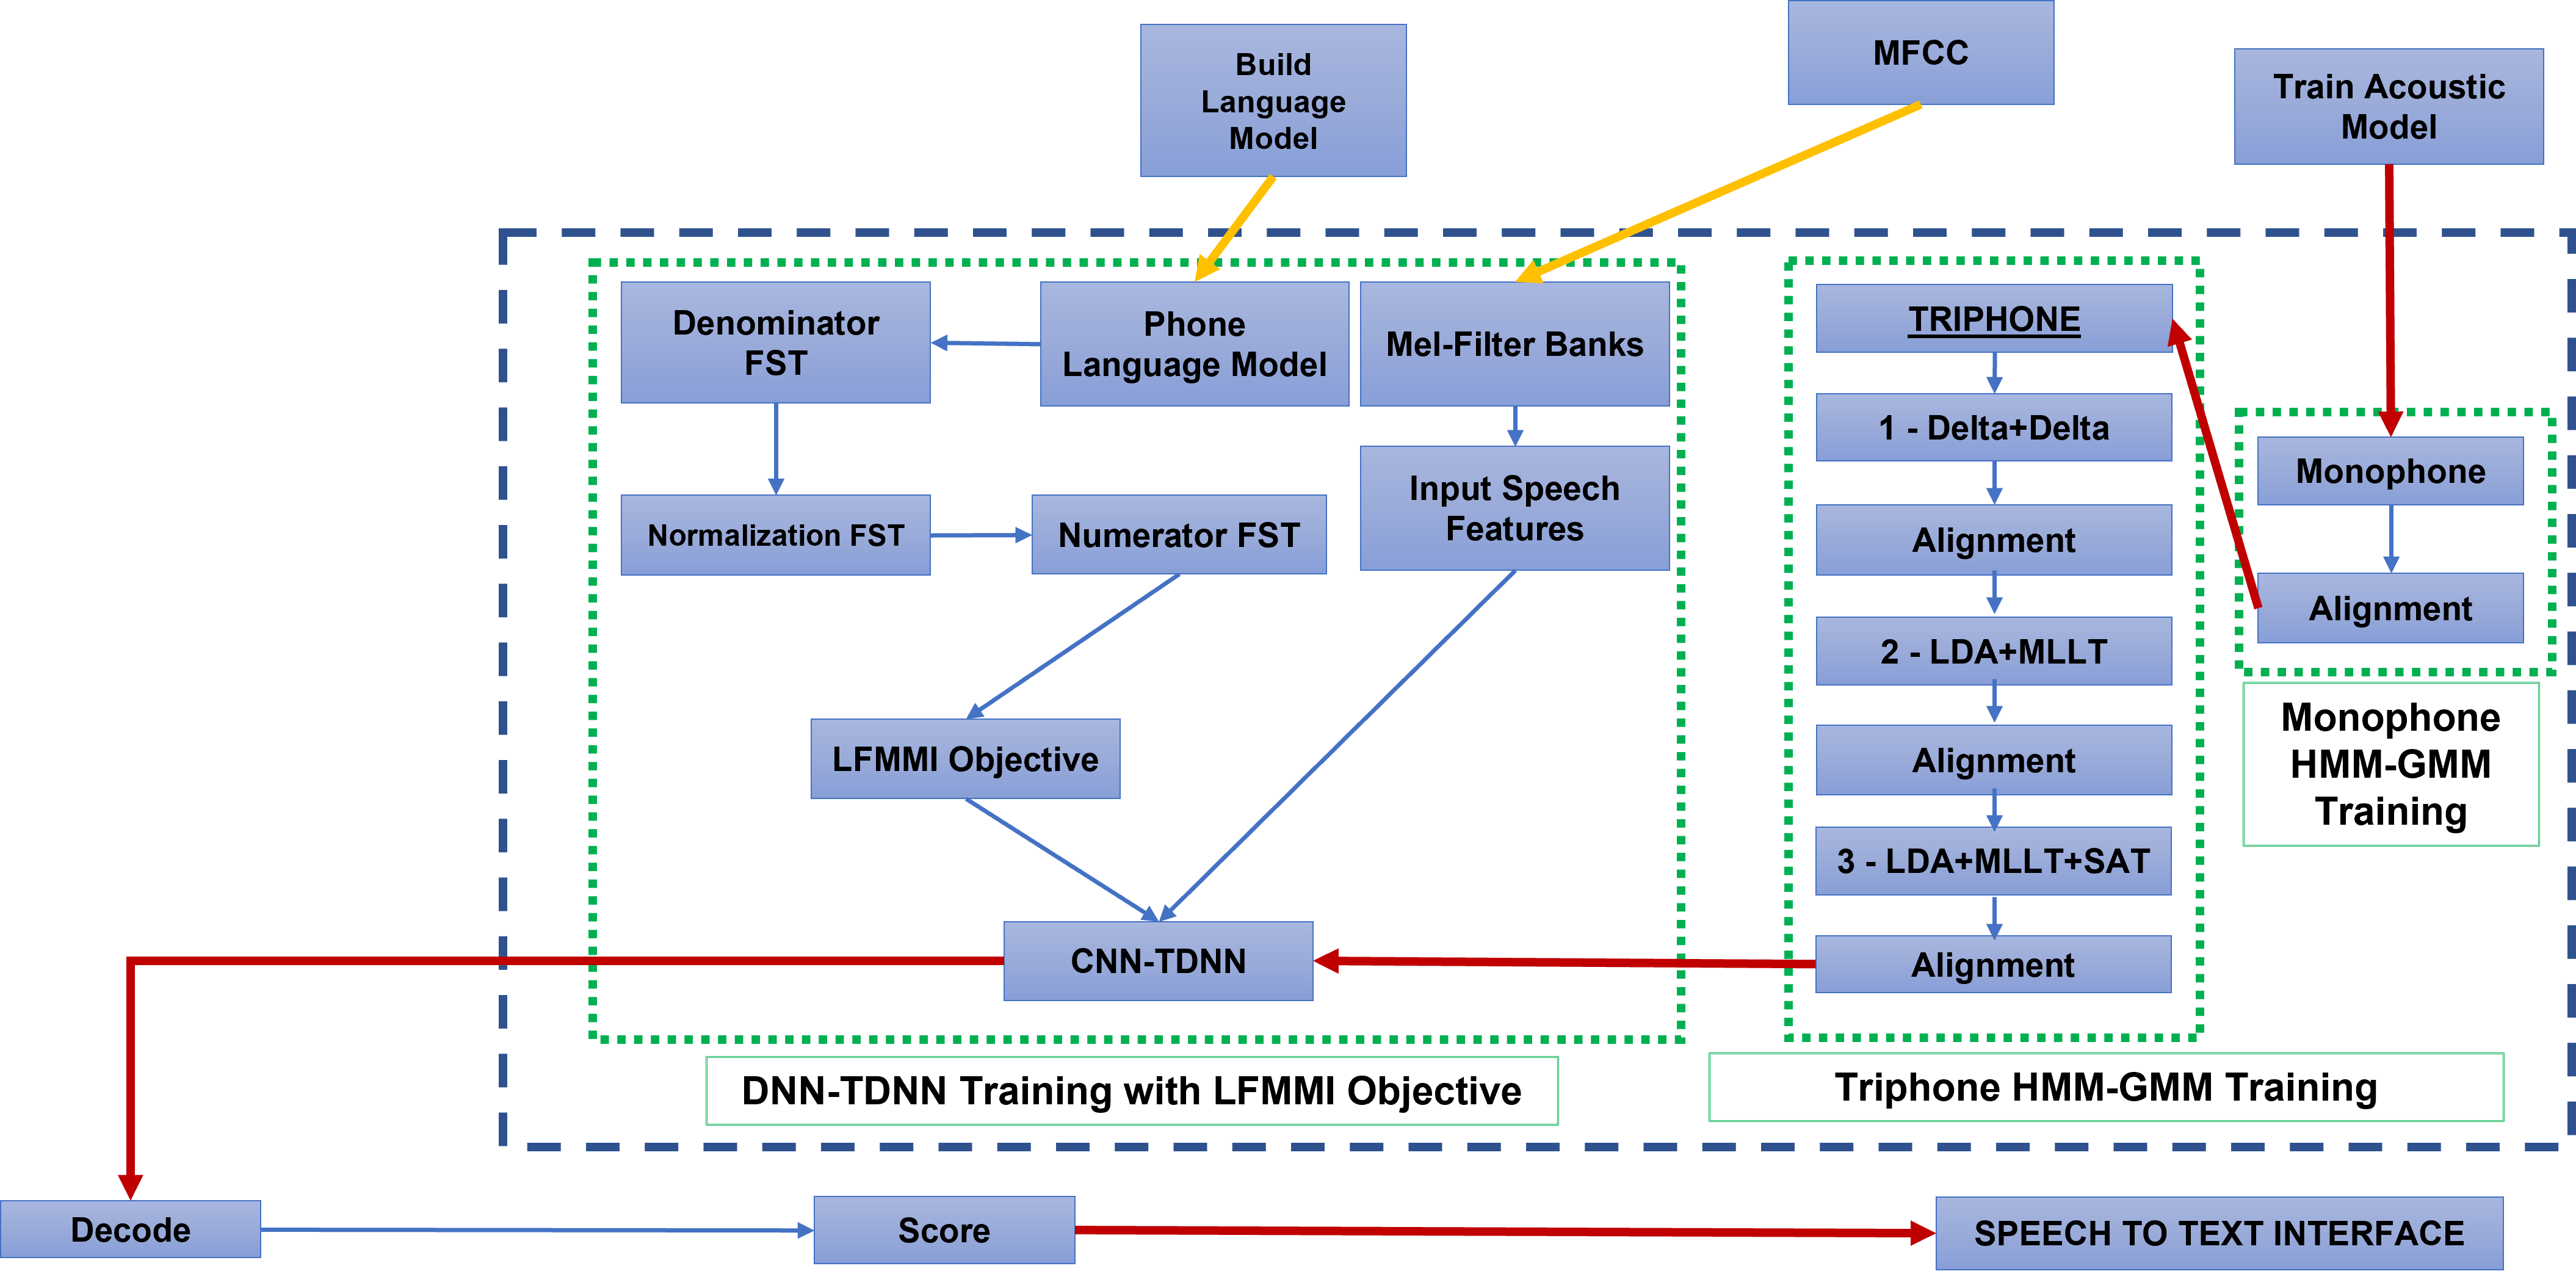
\includegraphics[width=0.95\textwidth]{img/Training-acoustic-model.png}
    \caption{Acoustic Modelling Workflow}
    \label{fig:acoustic-modelling-flow}
\end{figure}

\subsection{Mono-phone Training}
\label{sub:mono-phone}
The first step in training Acoustic Model for HMM-DNN system is to build a simple HMM-GMM acoustic model or mono-phone model in which the HMM states model context-independent phones which is used to force-align the training data-set so that rough estimates of phone boundaries can be obtained for a more complex model. %\cite{patil_automatic_2016} 

Mono-phone model does not include any contextual information about the preceding or the following phone and is used as a building block for the tri-phone models that utilize contextual information. %\cite{benesty_springer_2009}

After mono-phone training, we will align the audio with the acoustic models before moving on to the next training step, tri-phone training. The parameters of the acoustic model are estimated in acoustic training steps; however, the process can be improved by cycling through training and alignment phases, also known as Viterbi training. The Expectation Maximization and Forward-Backward algorithms are related but more computationally expensive procedures.

Additional training algorithms can improve or refine the model's parameters by using the output of aligning the audio to the reference transcript with the most recent acoustic model. As a result, there will be an alignment step after each training step in which the audio and text can be realigned. 

\subsection{Tri-phone Training}
\label{sub:tri-phone}
Phonemes will vary considerably depending on their particular context, while mono phone models represent simply the acoustic parameters of a single phoneme. The tri-phone models represent a phoneme variant within the context of two other phonemes (left and right). %\cite{benesty_springer_2009}

The data-set does not contain (and will never contain) all tri-phone units. There are three phonemes and thus three tri-phone models, but only a subset of those will appear in the data. To gather enough statistics for the data, the unit must appear multiple times in the data. A phonetic decision tree divides these tri-phones into fewer acoustically distinct units, reducing the number of parameters and making the problem computationally feasible.

In contrast to the mono-phone model, which compares each phoneme individually and assigns weights based on the probability of match, the acoustic parameters in tri-phone models are represented for a block of three consecutive phonemes. We can assign one HMM state from a total of 49 x 3 = 147  for each tri-phone. The training data-set, however, may not contain all of the tri-phones. A decision tree is used to group the tri-phones into a smaller set of distinct units.
%https://jonathan-hui.medium.com/speech-recognition-kaldi-35fec0320496

\begin{figure}[h]
    \centering
    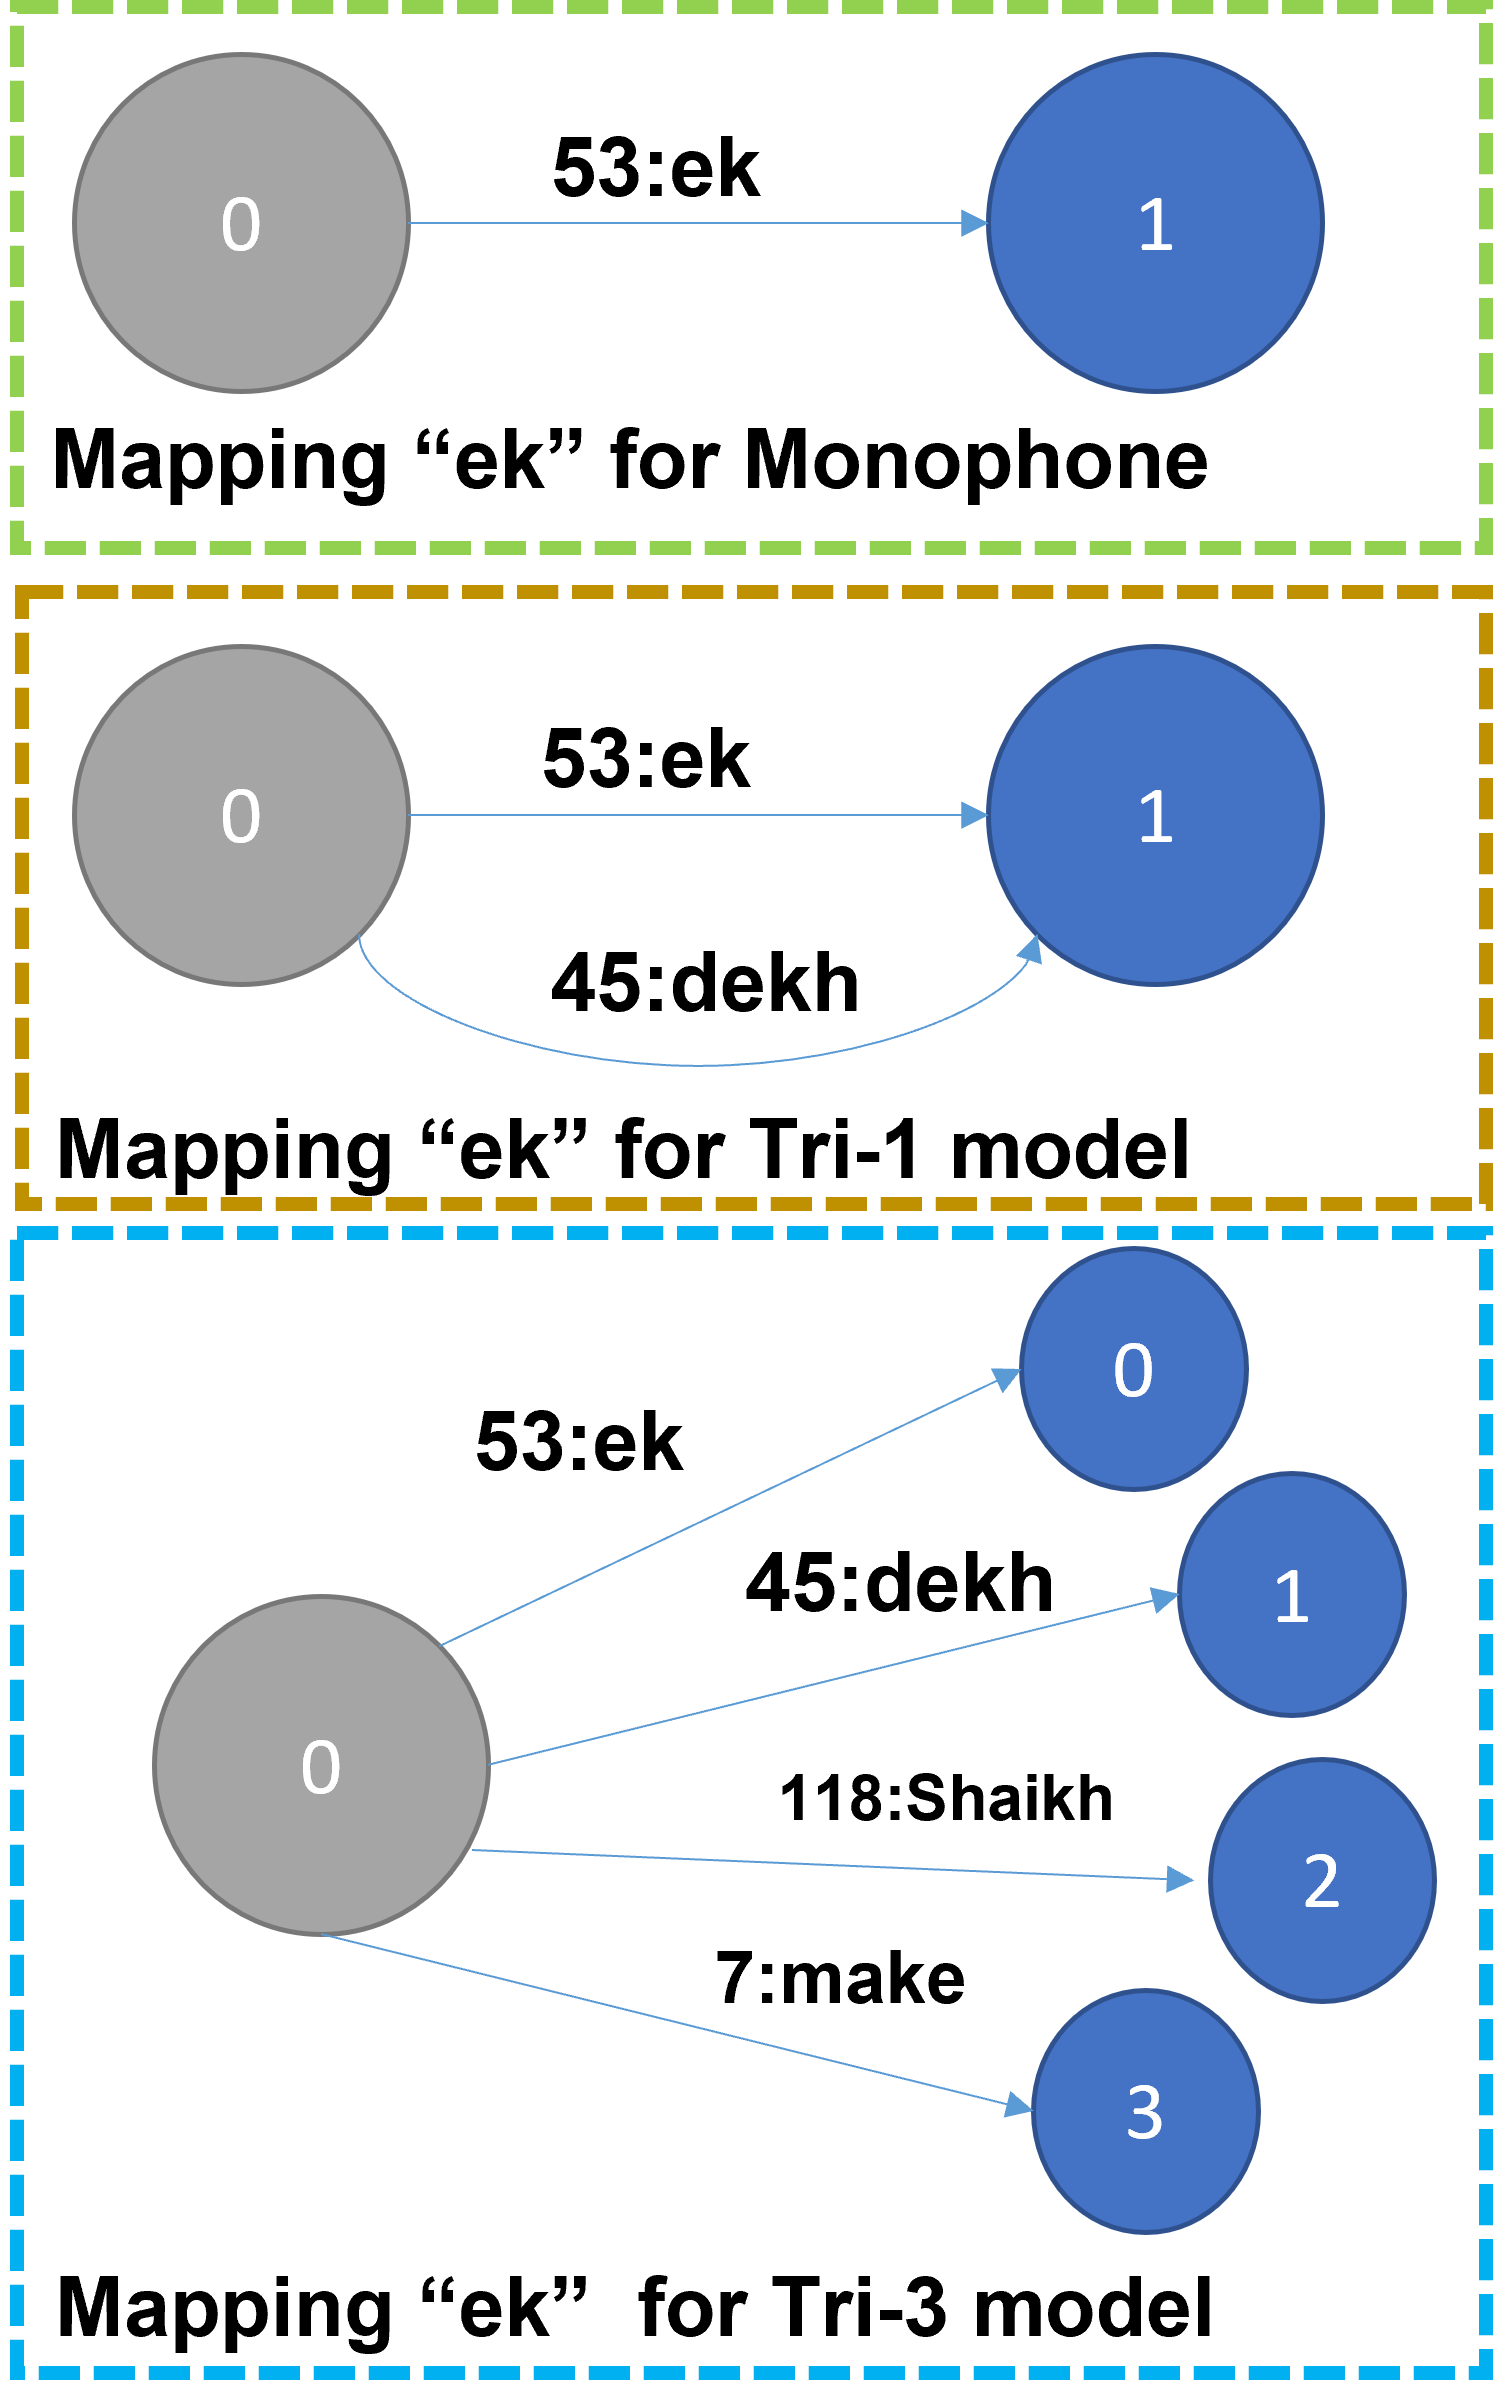
\includegraphics[width=0.4\textwidth]{img/mapping.png}
    \caption{Mapping the word 'ek' in mono-phone and tri-phone}
    \label{fig:mapping-mono-tri}
\end{figure}

The tri-phone model comprises of three types training models which we trained \cite{raj_note_nodate}:
\begin{enumerate}
    \item \textit{Delta and delta-delta training} - This training method computes delta and double-delta features, also known as 'dynamic coefficients,' in conjunction to MFCC features. They are the signal's first and second order derivatives (features). These characteristics are then used for recognition.
    \begin{itemize}
        \item In order to recognize speech better, dynamics of the power spectrum need to be understood i.e. the trajectories of MFCCs over time for which we use delta or differential and delta-delta or acceleration coefficients. 
        \item The delta coefficients are calculated using the following formula:
        \begin{equation}
        d_{t}=\frac{\sum_{n=1}^{N} n(c_{t+n}-c_{t-n})}{2 \sum_{n=1}^{N}n^2}    
        \end{equation}
        The delta coefficient from frame \textit{t} is represented by $d_{t}$ and is computed in terms of $c_{t-n}$ i.e. static coefficients to $c_{t+n}$. We usually take $n = 2$. Acceleration coefficients are similarly computed using differential instead of the static coefficients.
    \end{itemize}
    \item \textit{LDA-MLLT} - The most current TDNN-based architecture uses an \textit{"LDA-like transformation"} that is essentially an \textit{"affine transformation"} of the spliced input. LDA shrinks the feature space by generating HMM states for the feature vectors and the reduced feature space is used to create a transform that is unique to each speaker which is why MLLT is able to incorporate speaker independence.             
    \item \textit{Speaker Adaptive Training (LDA+MLLT+SAT)} - For each speaker, noise and speaker normalisation is performed using a data transform which enables the model to compute the variance due to the phoneme rather than the background environment using its parameters. 
    \begin{itemize}
        \item SAT also performs speaker and noise normalisation by adapting a particular data transform to each individual speaker. 
        \item The data, thus, becomes more homogeneous or standardised, allowing the model to focus its parameters on estimating variance due to the phoneme rather than the speaker or recording environment. Hence, this result has the lowest word error rate. 
        \item Following SAT training, the acoustic model is trained on speaker-normalized features rather than the original features. 
    \end{itemize}

\end{enumerate}

Audio is re-aligned with the acoustic models at the end of each tri-phone training before proceeding on to the next tri-phone model training step. In this step, the alignment algorithms include speaker-independent alignments and FMLLR. The Acoustic Model is no longer trained with the new normalised features after achieving the speaker-normalized features for SAT training. These partially speaker-independent models are used in the alignment process. Various scripts accept various types of acoustic model input but the actual alignment algorithm will always be the same. In the alignment process, speaker-independent alignment will exclude speaker-specific information. This training resulted in 13\% WER and 31.2\% SER.

\section{Neural Network Training with LFMMI Objective \\ Function}
\label{sec:LFMMI-chain}
The DNN model, which introduces the concept of unsupervised training or adaptation, eliminates the need to provide adaptation data in advance. Hence we will enhance our system by modelling the acoustic units with DNN rather than using GMMs. For Neural Network Training, we used Chain CNN-TDNN with LF-MMI as the objective function. The Chain model is outlined in Figure \ref{fig:Chain-Training-outline}.

\begin{figure}[h]
    \centering
    %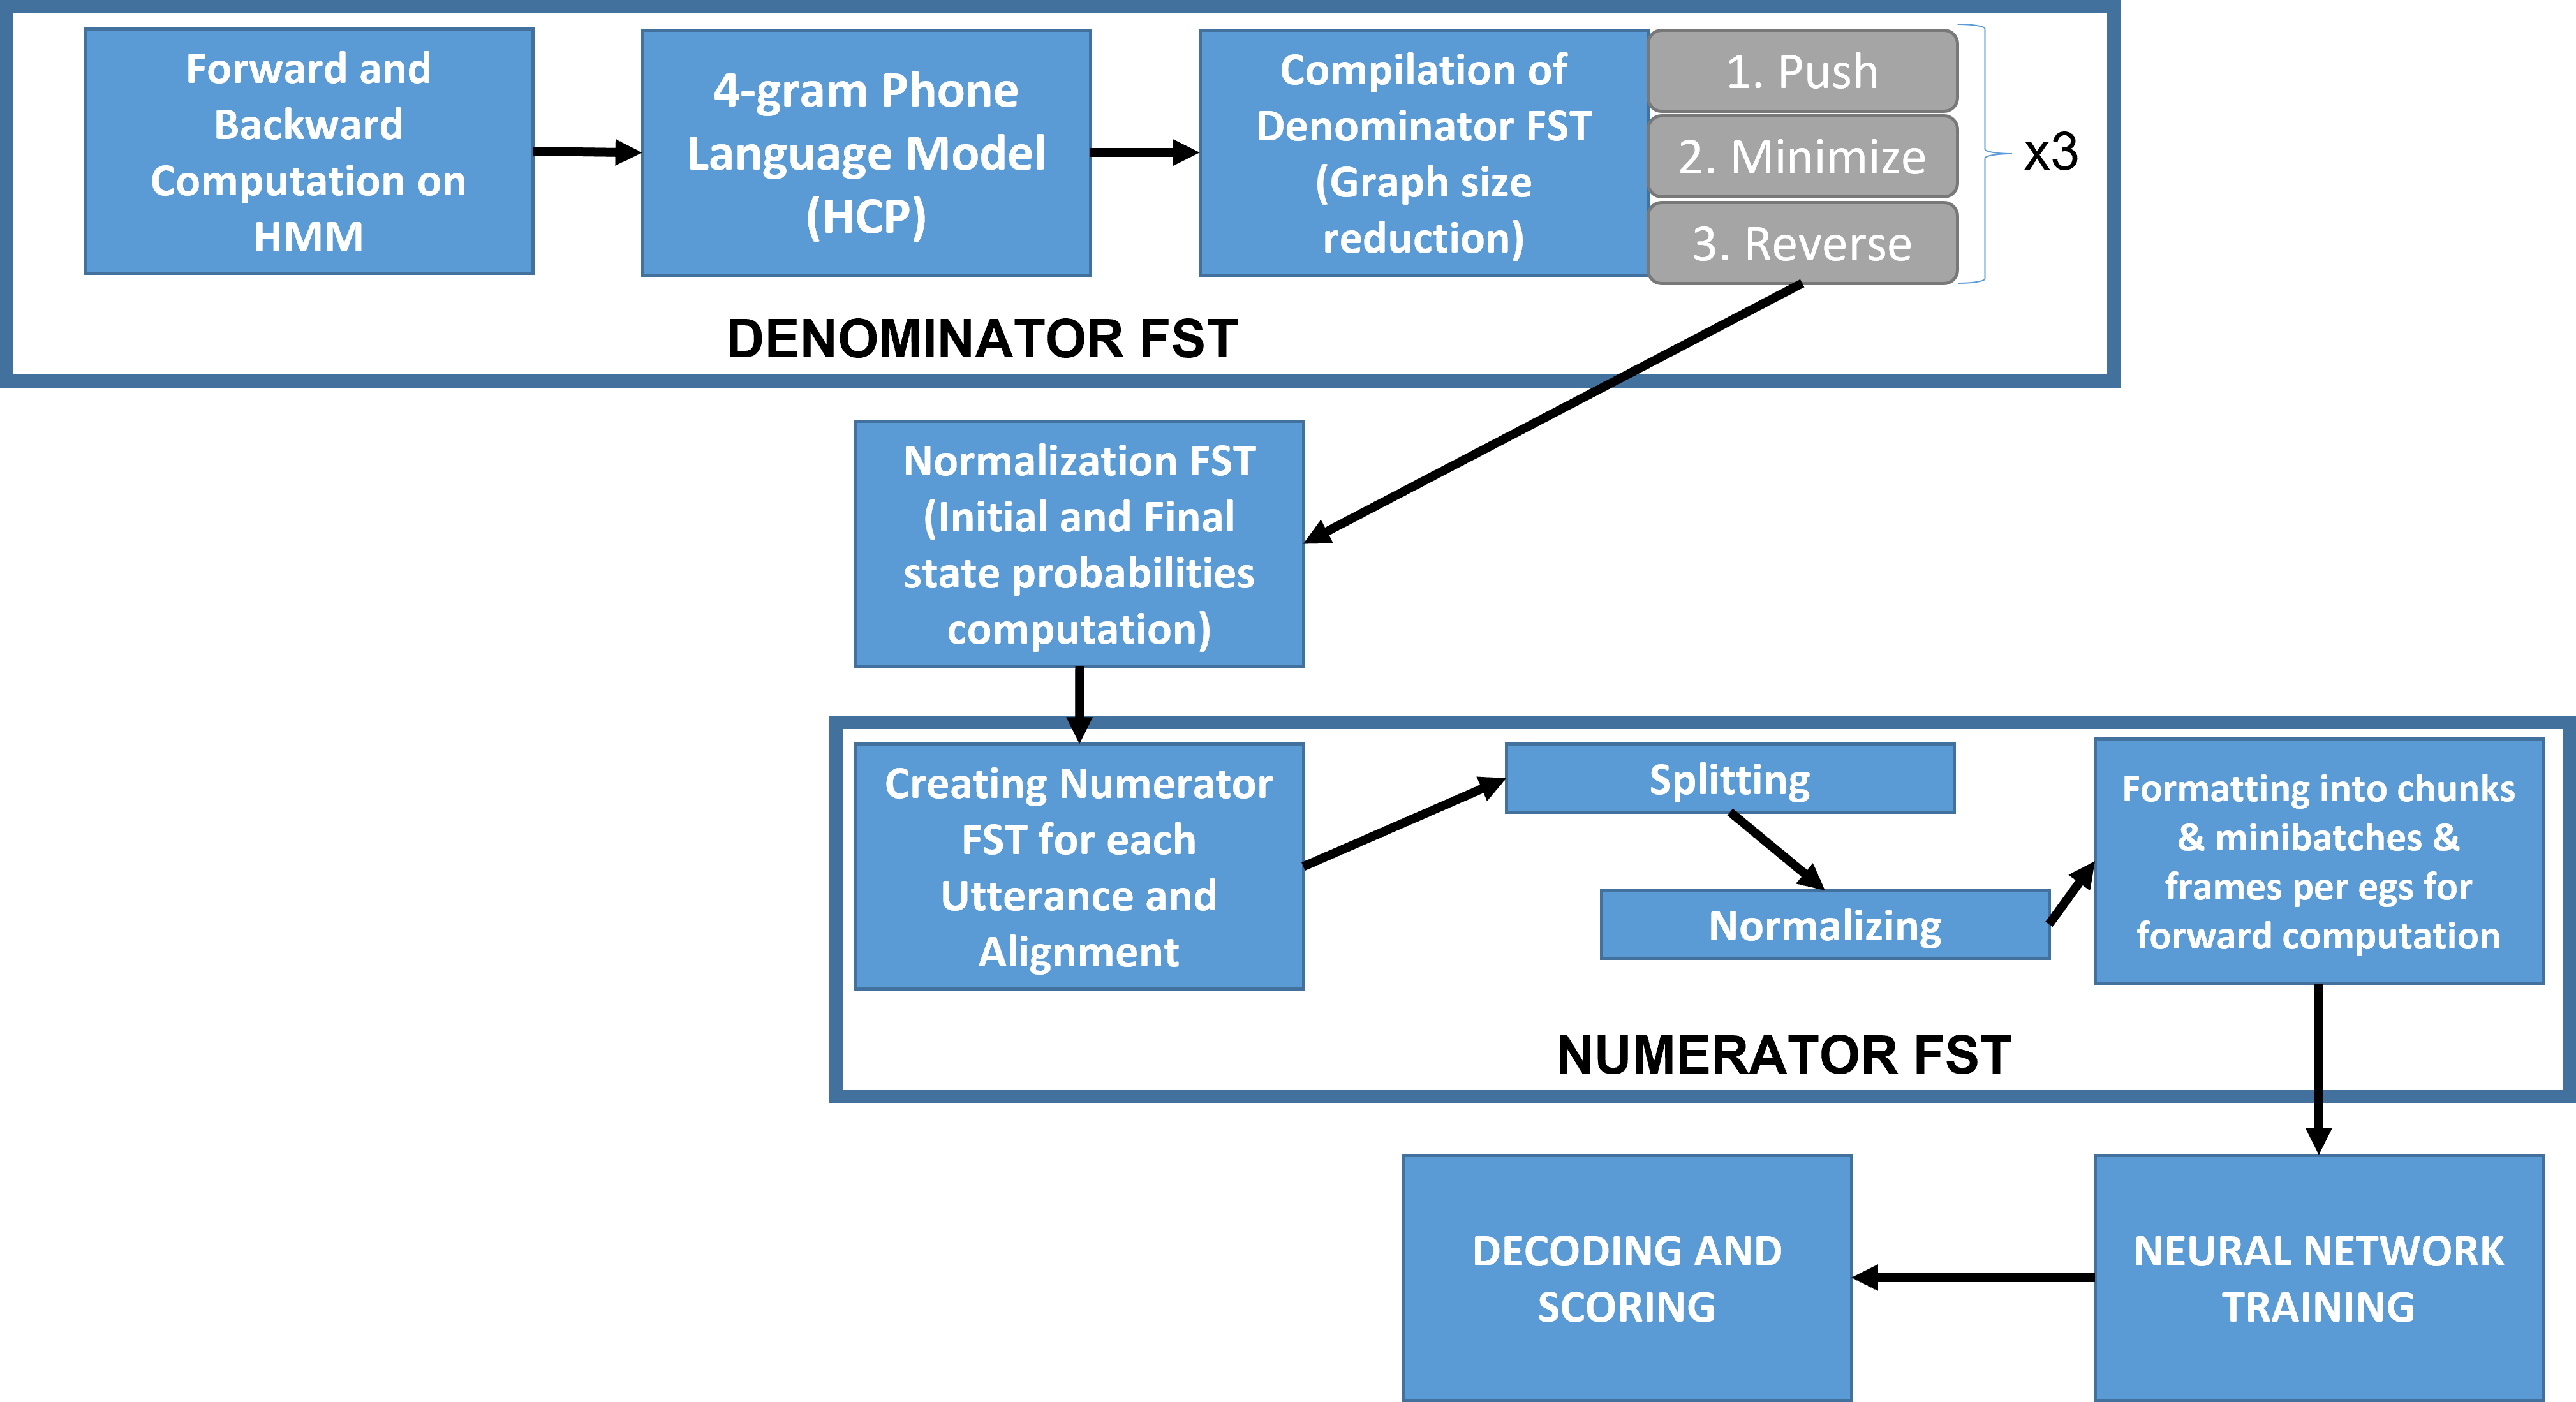
\includegraphics[width=0.8\textwidth]{img/ChainTrg.png}
    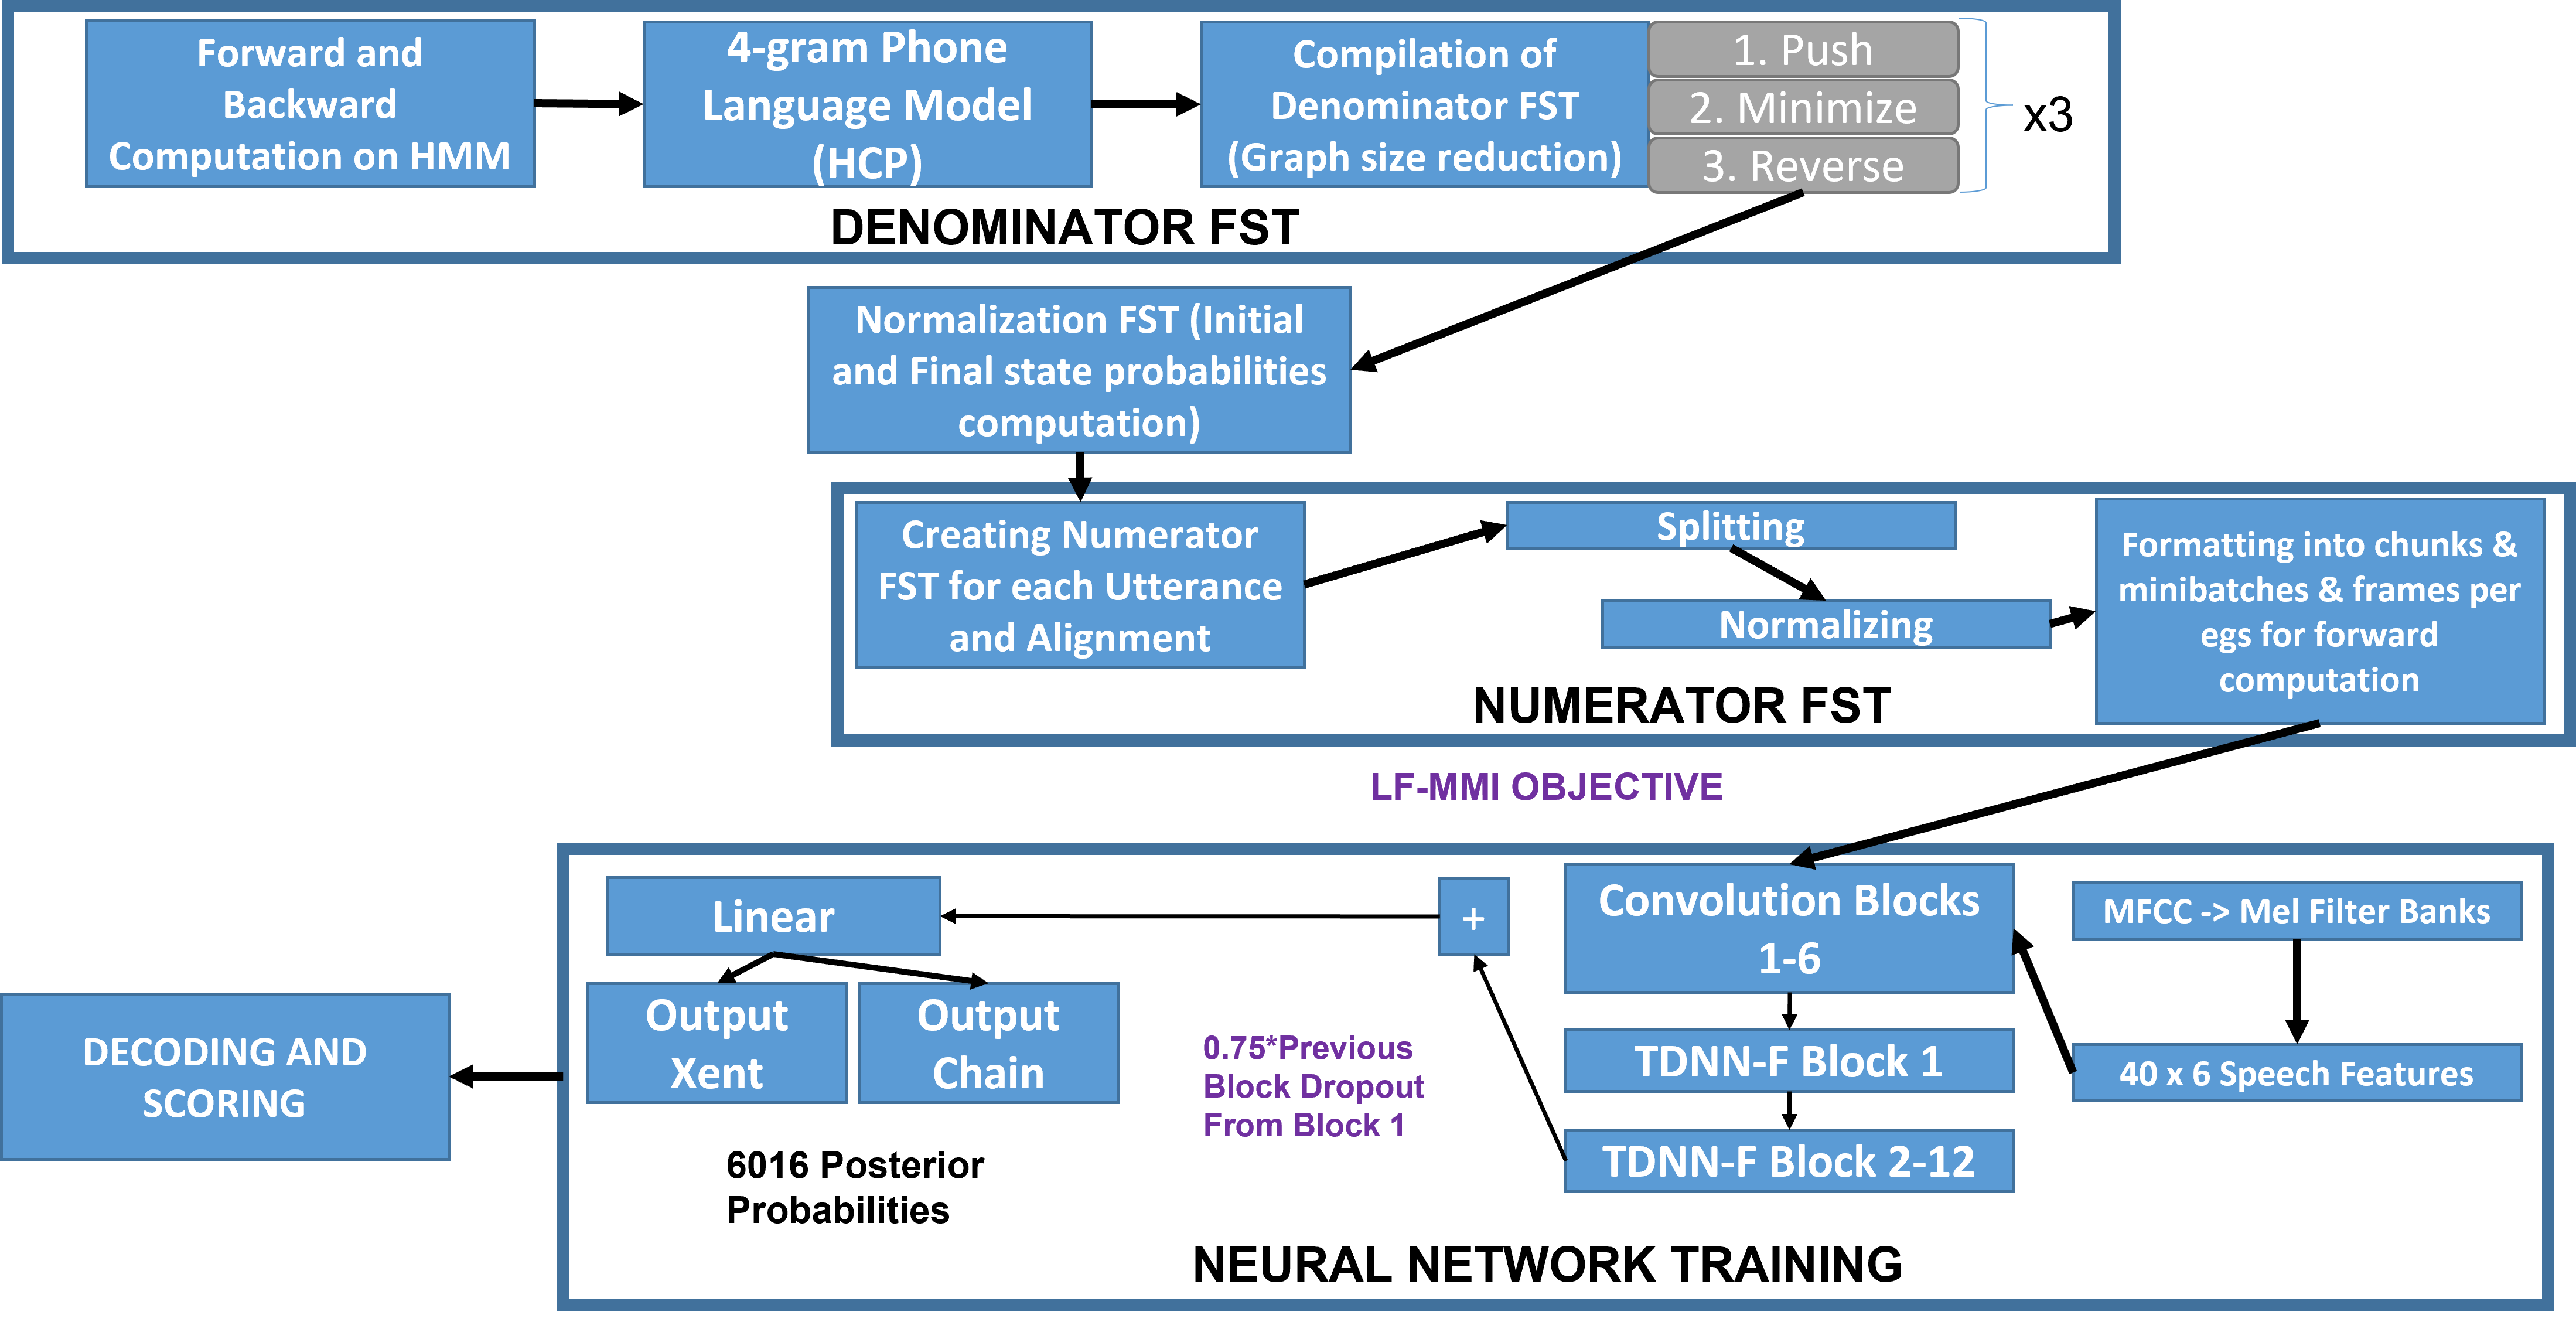
\includegraphics[width=0.95\textwidth]{img/ChainModel-Detail.png}
    \caption{Chain or LFMMI Training Outline}
    \label{fig:Chain-Training-outline}
\end{figure}
 

\subsection{LFMMI Objective Function}

The chain model or Lattice Free Maximum Mutual Information Model is like a typical HMM-DNN with one third of the traditional frame rate at the DNN's output. The DNN's input features are at the original frame rate of 100 frames per second since CNNs, LSTMs, TDNNs, etc have recurrent connections or splicing inside them and are they are not purely feed-forward nets. This model uses a frame-level objective i.e. log-probability of the correct phone sequence. 

The initial probabilities of the corresponding FSTs requires re-adjustment since the utterances are split into 1.5 second slices. Utterances are sliced off often from the middle. This initial probability is calculated by performing the HMM for 100 time-steps beginning with the initial state and then averaging the distribution of states over these 100 time-steps.

The HMM should be traversable in a single transition of a model at the normal frame rate instead of three transitions. A single-occurring state is present in the current topology, followed by a state that can appear zero or more times. Similar to GMM-based models, the state-clustering is obtained, but with a different topology for converting the alignments to the new topology and frame-rate.

Chain model training process is a lattice-independent version of MMI, in which a forward-backward algorithm over an HMM created from a phone-level decoding graph is used to obtain the denominator state posteriors. A similar forward-backward algorithm, but restricted to transcript-corresponding sequences, is used to obtain the numerator state posteriors.

Like MMI, numerator and denominator 'occupation probabilities' computed and the difference between the two is used in the derivative computation. Normalization of DNN outputs is no longer required to sum to one on each frame as it makes no difference. A modified HMM topology is used because of frame rate of 1 frame per 30 ms \cite{daniel_povey_kaldi_nodate}. The gradient descent requires computation of two sets of posterior probabilities for: 
    \begin{enumerate}
    \item Numerator graph specific to an utterance 
    \item Denominator graph encoding every possible word sequences which will be the same for all utterance in LF-MMI unlike the lattice-based MMI. 
\end{enumerate}

Forward and backward computations are computed in these two situation:
\begin{enumerate}
    \item During training time for computation of numerator FST and denominator FST state occupancies which are the product ($\alpha \beta$) of any states obtained using forward ($\alpha$) and backward algorithm ($\beta$) respectively.
    \item During Testing time Veterbi Decoding while pruning FST some type of forward looking is required to avoid pruning paths that can have higher probability at later stage using $\beta$ as a proxy look-ahead. 
\end{enumerate}

The forward and backward computations for numerator FST are on CPU since they are small and for denominator FST, these computations are performed on GPU but not on log domain since computation of log several times slows the process. The objective function values can occasionally become bad for which we keep the objective function within [-30,30] range \cite{raj_experiments_nodate}. To reduce the maximum memory usage, the denominator computation is performed before the numerator. This algorithm is also prone to numeric overflow and underflow, which can be avoided by multiplying the emission probability of the frame by the normalisation factor $\frac{1}{alpha(t)}$.

Now we will explore the key processes in the chain model.

\subsubsection{Forward and Backward Computation of Denominator FST} 

A derivative of the form \textit{"numerator occupation probability - denominator occupation probability"} for each output index or pdf-id of the Neural Network is computed and propagated back into the Neural Network. 
    \begin{itemize}
        \item Forward-backward over an HMM for the denominator is done as part of the computation. 
        \item The labels or pdf-ids are associated with the arcs rather than the states because it is represented as a finite state acceptor. 
        \item Although this is not a true traditional HMM, it is still regarded as one due to the use of the forward-backward algorithm (denominator FST) to obtain posteriors.
    \end{itemize}    
\subsubsection{Phone LM \& Denominator FST} 
Building Phone LM is first step to build the denominator FST. 
    \begin{itemize}
        \item Phone LM is derived from phone alignments in training data making it an un-smoothed language model, which means there is no reverting to lower order n-grams. 
        \item Transition to some LM states that are removed go to lower order n-gram states. Smoothing is avoided to reduce number of arcs in compiled graph after phonetic context expansion.
        \item There is a requirement for maintenance of 2-phone history which is why a 4-gram language model is used for chain training and we never prune LM states below the trigram level which not pruned because any sparsity in which trigrams are permitted tends to reduce the size of the compiled graph.
    \end{itemize}

%In addition to the number of states dictated by the no-prune trigram rule, we have a selectable number (e.g., 2000) of 4-gram language model states to be retained (the rest are identified with the corresponding trigram state), and the ones we select are determined in a way that maximises the training-data likelihood. To maximise the training-data likelihood, all probabilities are estimated. 

%It is worth noting that if our phone LM was just a simple phone loop (i.e. a unigram), it would be expanded to triphones due to phonetic context effects, but it would contain arcs for all possible trigrams. So any sparsity obtained by using the un-pruned trigram model is a bonus. Empirically, an un-smoothed trigram LM is what expands to the smallest possible FST; and pruning some of the trigrams results in little or no WER improvement while increasing the size of the compiled FST (at least on 300 hours of data expanded 3-fold with speed perturbation; on less data it might help). 

%The phone-LM perplexities for the various models we tried on the Switchboard setups ranged from 5 to 7; the phone-LM perplexity with our chosen configuration (4-gram, pruned to trigram for all but 2000 states) was around 6. Lower phone-LM perplexity did not always result in better WER of the trained system; for conventional (word-based) MMI training, an intermediate strength of language model seemed to work best.

\subsubsection{Compilation of the denominator FST} 
Phone LM is expanded into an FST with pdf-ids as the arcs, through a process akin to a normal decoding-graph compilation, but without using a Lexicon, at end of which the transition-ids are converted to pdf-ids. 
    \begin{itemize}
        \item The difference lies in graph size minimization because the standard recipe calls for determination and minimization. 
        \item This procedure it's variants with disambiguation symbols, do not allow graph size reduction which is why the graph-minimization procedure is three repetitions of: 
        \begin{enumerate}
            \item Push
            \item Minimize
            \item Reverse (The terms 'push' and 'reverse' refer to reversing the directions of arcs and swapping initial and final states.)
        \end{enumerate}
    \end{itemize}
    
\subsubsection{Initial \& Final Probabilities} 
A starting state and final probabilities for every state are produced by the graph-creation process naturally. 
    \begin{itemize}
        \item These are not the states used in the forward-backward procedure because these probabilities apply to utterance boundaries but it is trained on fixed-length chunks of utterance which is usually 1.5 seconds. 
        \item Constraining the HMM to the initial and final states at these arbitrarily chosen cut points is not appropriate. 
        \item For each state instead, we use: 
        \begin{itemize}
            \item Derivation of Initial Probabilities from fixed iterations of HMM-running 
            \item Averaging the probabilities
            \item Final probabilities = 1.0 for each state.
        \end{itemize}        
    \end{itemize}    

\subsubsection{Normalization FST} 
The initial and final probabilities are applied to the initial and final frame as part of the computation in the denominator forward-backward process. 
    \begin{itemize}
        \item Normalisation FST is a version of the denominator FST with these initial and final probabilities. 
        \item Epsilon ($\epsilon$) arcs are used to simulate initial probabilities since they are unsupported by FSTs. 
        \item Probabilities will then be added to normalization FST using Normalization FSTs.
    \end{itemize}   
    
\subsubsection{Numerator FSTs} 
A numerator FST for each utterance is generated to prepare the training process, which encodes the supervision transcript along with the transcript alignment to force similarity to reference alignment, allowing a little deviation, acquired from a base-line system . 
    \begin{itemize}
        \item A phone is allowed  in the lattice alignment to occur 0.05 seconds prior or after its start and end positions, respectively. 
        \item Alignment details must be included as training is done on fixed-length utterance segments rather than complete utterances, i.e. If we know where the transcript aligns, we can split the utterance into pieces, which is important for GPU-based training.
        \item Rather than enforcing a specific pronunciation of the training data, a lattice of alternative pronunciations of the training data is used, which is generated by a lattice-generating decoding procedure that uses an utterance-specific graph as our reference decoding graph, generating all pronunciation alignments within a beam of the highest-scoring pronunciation.
    \end{itemize}

\subsubsection{Splitting the numerator FST} 
Fixed sized utterances of 1.5 seconds length are used, necessitating division of the numerator FSTs into fixed-size segments. This is simple because the numerator FSTs remembers and encode time-alignment information and  have a structure that allows association of any FST state with a specific frame index. At this time, there are no costs in the numerator FST. It is only viewed as encoding a path constraint, so there is no need to decide how to split up the costs on the paths.

\subsubsection{Normalizing the numerator FSTs} 
Normalisation FST is merged with split-up pieces of numerator FST to ensure that the denominator FST costs reflect in the numerator FST which in turn ensures that objective functions are never positive and making their interpretation easier. 

This prevents the objective function from ever decreasing by preventing the numerator FST from having state sequences that the denominator FST would find unacceptable while also protecting against the possibility of numerator FST containing state sequences not accepted by denominator FST, which allows the objective function to indefinitely increase. 

The Lattices may contain n-gram phone sequences which were not seen in training since Phone LM has no smoothing and is estimated from 1-best alignments. Normalization process infrequently generates empty FSTs which can happen when: 
        \begin{itemize}
            \item The lattice consists of tri-phones absent in the 1-best alignment that was used to train the Phone LM and, 
            \item No alternative paths are available at that point in the lattice to compensate for the resultant failed paths which is a possibility because the lattice-producing alignment and 1-best alignment selected different pronunciations of the same word which is why These utterance fragments are simply discarded.
        \end{itemize}

The initial probabilities are now have different values which becomes a problem for chunk-level FSTs. To approximate this, the HMM running is done for a few iterations and then the probabilities are averaged to be used as the initial probability of any state. Thus Normalization FST seems to work despite being a crude type of approximation. The numerator FST is composed with the normalization FST for following reasons: 
       \begin{enumerate}
            \item Ensure that objective function value is always negative for easier interpretation. 
            \item Ensure that the numerator FST is free of sequences not permitted by the normalisation or denominator FST, which commonly happens because the sum of the overall path weights for such sequences is dominated by the normalization FST part. %\cite{raj_experiments_nodate}.
        \end{enumerate}

\subsubsection{Format of the numerator FSTs} 
Pdf-ids can not be directly used as weighted acceptors in the numerator FSTs because they could be zero which is treated differently by Open-Fst i.e. as epsilon. Hence, numerator FSTs' weighted acceptors correspond to \textit{"pdf-ids + 1"}. Instead of storing an array of separate numerator FSTs, they are appended together to form a longer FST when mini-batches are formed. This enables a single forward-backward algorithm to be applied to every utterance in the mini-batch, directly calculating the total numerator log-probability. 

\subsubsection{Chunks-Size} 
The number of output frames for each chunk of data that we analyse and evaluate during training or decoding is known as the chunk-size.
    \begin{itemize}
        \item There is a mechanism for variable chunk sizes that permits reasonably large chunks while preventing data loss from files that are not exact multiples of the chunk size. 
        \item The first specified chunk size is called primary chunk-size which is unique because we can choose no more than two non-primary chunk sizes for any given utterance and the remaining chunks must be of the primary chunk size. Determining the optimal split of a file of a given length into chunks is made easier by this restriction, allowing the biasing of chunk-generation to chunks of a specific length.
        \item The number of frames per chunk influences the speed or latency trade-off but not the results.
    \end{itemize}    

\subsubsection{Mini-Batches} 
A larger mini-batch size is generally more efficient because it interacts well with optimizations used in matrix multiplication code, particularly on GPUs, but it can lead to update instability if it is too large and the learning rate is too high. %We used mini-batch of 64 based on our dataset scenario. %Size 512 for GPU-based training is recommended and was used.
    \begin{itemize}
        \item To reduce the size of the denominator FST for training on the GPU training is done on 1 to 1.5 seconds chunks, instead of the complete utterance. However, the transcript needs to be broken up to do this and 1-second chunks may not coincide with word boundaries.
        \item Utterances are divided into given fixed-length chunks of speech to train on mini-batches of length 1.0 seconds. 
        \item Shorter utterances are removed, while longer utterances are divided into chunks with small gaps or overlaps between them.
        \item The acoustic models usually require left or right frames for acoustic context which is added but the context is added after the chunks have been determined. 
        \item Usually the mini-batch size is a power of two, and is possibly limited by GPU memory constraints. We used 64 mini-batches based on our data-set. 
        \item The alpha probabilities in forward-backward computation consume the most GPU memory. 
        \item After the 3-fold sub-sampling, we have 50 time steps with a 1 second chunk.
    \end{itemize}

\subsubsection{Frames per Egs} 
The entire data-set is randomised at the frame level for the most basic types of networks, such as feed-forward networks or TDNNs trained with the cross-entropy objective function, and training is done on one frame at a time. 
    \begin{itemize}
        \item Data is pre-randomized at the frame level in order for the training jobs to mostly do sequential I/O. 
        \item If 10 frames are needed each of left and right context or when generating the training examples, there may be a requirement of increasing the amount of data by a factor of 20. This issue is resolved by including labels for time value ranges i.e. \textit{frames-per-eg} value, and include enough left/right context that we can train on any of those given frames. If that value is suppose 10, any given training job will pick one of those 10 frames to train on. 
        \item Based on our data-set and scenario we used values of 150,110,100,30 for \textit{Frames per Eg}.
    \end{itemize}
 

%We used Frames per e.g = 150, 110, 100, 30 due to varying size of our data-set and 10 Epochs and Initial Number of jobs =3 and Final Number of jobs= 16 for trainer optimization.  

%https://kaldi-asr.org/doc/dnn2.html
%https://kaldi-asr.org/doc/chain.html

\subsubsection{Avoiding Over-fitting}
To avoid over-fitting, LF-MMI uses following techniques \cite{raj_experiments_nodate}:
\begin{enumerate}
    \item \textbf{L-2 regularization on neural network outputs:} This forces the weight parameters to decay or approach zero but become exactly zero. It is also called Ride Regression or Weight Decay. Smaller weight parameters makes neurons negligent which reduces neural network complexity and hence, over-fitting. 
    \item \textbf{Separate classifier Output Layers:} LFMMI uses two separate output layers for classifier, one trained with MMIE and the other with cross-entropy so that the overlapped layers will be trained with both objectives to reduce over-fitting that is caused by a single objective.
    \item \textbf{Multitask training with the cross-entropy objective:} The forward probabilities at each time step in the numerator graph are used as soft targets instead of the usual hard targets.
    \item \textbf{Leaky HMM:} This permits small transition probability between any two states is allowed allowing for gradual context forgetting. %https://m-wiesner.github.io/LF-MMI/
\end{enumerate}

\begin{figure}
    \centering
    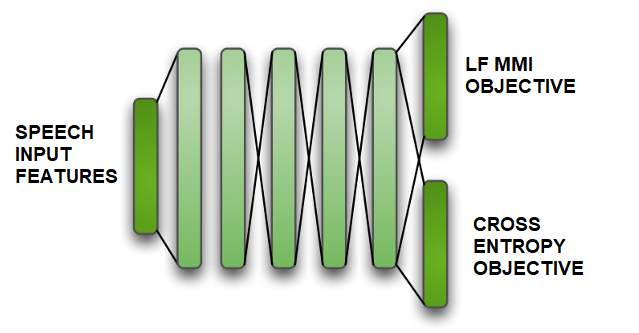
\includegraphics[width=0.7\textwidth]{img/LFMMI-crossent.png}
    \caption{LFMMI input objectives}
    \label{fig:LFMMI-INPUT}
\end{figure}

\subsection{Neural Network Training with CNN-TDNN}

For The Neural Network training part in Figure \ref{fig:Chain-Training-outline} the 1500ms speech segments with 40 Mel filter-banks features and 200 iVectors are the input and structure of the network is CNN-TDNN as shown in Figure \ref{fig:CNNTDNN-Layout}. The LF-MMI here is the training objective i.e. they define how the weights are set during the training. We will now explore this further.  

We will use CNN-TDNN for Neural Network training because various reports like \cite{abdel-hamid_convolutional_2014}, \cite{zorila_investigation_2019}, \cite{biswas_semi-supervised_2019}, \cite{noauthor_tdnn_nodate} \cite{georgescu_kaldi-based_2019} and \cite{kreyssig_improved_2018} suggested that CNN-TDNN perform better than simple TDNN, however, the former requires relatively a bit more computing power \cite{georgescu_performance_2021} which is very minor. 

\cite{georgescu_kaldi-based_2019} conducted a comparative test of various TDNN based architectures on RSC and SSC Datasets. The RSC corpus consisted of read speech utterances recorded in a silent environment whereas SSC corpus comprised of spontaneous utterances, gathered from the Romanian media broadcasts of which some were clean, recorded in a silent environment, while the others contained background noise. Their results showed that CNN-TDNN performed better with the noisy SSC corpus which made it perfect for our use.

The performance of various HMM-DNN and E2E architectures were investigated by \cite{georgescu_performance_2021}, which shows that it performed almost equally to TDNN in a clean data-set of Librispeech but on "other" data-set of LibriSpeech, CNN-TDNN actually performed better than pure TDNN and E2E models. 

CNN-TDNN is a variant of simple TDNN model and it is part of a multi-component system comprising of a hybrid HMM-TDNN based acoustic model, a phonetic model and an n-gram language model. Optionally for re-scoring, a complex n-gram or NN-based LM can be used. In Chain or LFMMI model with CNN-TDNN, 4-gram model is used. 

Mel-filter-banks are used in this implementation instead of MFCCs, in terms of network input features. Here the final features are organized as a matrix unlike simple TDNN where the input features are represented as a vector. 

The input in the CNN-TDNN network comprises of two feature types organized in a 40x6 matrix of speech features \cite{georgescu_performance_2021}: 

\begin{enumerate}
    \item 40-dimensional Mel-filter-banks extracted from 25 ms length frames
    \item 200-dimensional and 10 ms i-vectors-shift calculated from chunks of consecutive 150 frames
\end{enumerate}

The feature extraction procedure and organization of these features are shown in Figure \ref{fig:CNN-TDNN-INPUT}. TDNNs are one dimensional or temporal CNNs whereas CNN works on time as well as frequency dimension. Note that unlike TDNN, CNN-TDNN requires Mel filterbanks instead of MFCCs because the CNN layer needs to have a meaningful non-time dimension to operate on which is why we want our signals to be in  frequency space or dimension. They are still dumped to disk as MFCCs during the NN extraction and training process but the DCT part of MFCC is inverted or reversed to get Filterbanks. 

The neural network component acoustic model of CNN-TDNN resembles TDNN, the key difference being placing of few CNN layers prior to the time-delay layers, acting as a front-end block. The input for Conv. Block 1 are three matrices of speech features i.e. the features for the current, previous, and next acoustic frames, or a feature volume of 6 x 40 x 3 equivalently. Time and feature space convolutions are performed using 64 filters of size 3x3, and the output is 64 x 40 x 1 volume. %\cite{georgescu_performance_2021}

The Second Convolutional Block's input comprises of three time consecutive volumes as the first Convolutional Block's output, that are spliced together to form the 64 x 40 x 3 feature volume. The second Convolutional block performs time and feature space convolutions with another 64 3x3 filters and gives 64 x 40 x 1 volume as output. 

In Convolutional Blocks 3–6 more filters are used, ranging from 128 to 256, while feature volume size is kept constant by reducing the height from 40 to 20, and then to 10, finally generating a 2560-dimensional output that is passed on to the next time-delay blocks from whereon the processing is same as TDNN.

Convolutional layers have the property of annihilating small variations in the spectral domain due to their structure provided by local connectivity, weight sharing, and pooling \cite{georgescu_performance_2021}. These variations are induced by both the speaker and the acoustic environment in which the speech takes place. 

The Convolution Block 2 input has three time consecutive volumes as the Convolution Block 1 output, spliced together to form the 64 x 40 x 3 feature volume. The second convolutional block performs time and feature space convolutions with another 64 3x3 filters and gives a 64 x 40 x 1 volume as output.

Conv. Blocks 3–6 more filters ranging from 128 to 256, while maintaining the size of the feature volume by reducing the height from 40 to 20, and finally to 10. The convolutional blocks generate a 2560-dimensional output that is passed on to the following time-delay blocks. %\cite{georgescu_performance_2021} 

The possible reason why adding CNNs before TDNN improves performance in noisy environment is that TDNNs are basically time-dilated 1 Dimensional CNNs and if the input features are noisy, having a few CNN layers (2D CNN) at the input would help the model learn some non-linear transformations which can reduce the effect of the noise on speech input. %(think of the D dimension in the input).

Front End CNN Blocks are followed by 12-blocks of factored TDNN (TDNN-F). TDNN-F Block 1 processes the current time frame only, while the rest perform temporal convolution over $t-3$, $t$, and $t+3$  time indexes. The linear layer is formed by splicing the input vectors at time indexes $t-3$ and $t$ are spliced together to form the linear layer. The affine layer is formed by splicing the input vectors at time indexes $t$ and $t+3$.  

TDNN employs a sub-sampling technique to compute hidden activations only at specific time steps which avoids redundancy because the large overlap of contexts leads to highly correlated neighbouring activations. A larger context on the left side is usually found to be optimal for online decoding. This way, Model size and training time are reduced. 

TDNN with sub-sampling increases training speed and are therefore faster than LSTM. They learn local correlations between speech frames. Bottleneck layers, which are initialized by Singular value decomposition (SVD), constrains rank of weight matrices which help in regularization and reduces number of Multiplications $M x N -> (M+N) x R$. 

The TDNN network's sub-sampling mechanism is similar to a convolutional operation that allows gaps in the convolutional filter which is another network variant based on the purely TDNN approach, with a couple of stacked convolutional layers added before with a primary function to further process acoustic features and act as a feature processing front-end. These additional layers reduce spectral and temporal variability. 

The output blocks use cross-entropy and chain loss functions in TDNN and CNN-TDNN both. The CNN-TDNN and simple TDNN architectures have identical Neural Network output blocks, which are represented by 6016-dimensional posterior probabilities of acoustic states, while the language model of 200K words provides the system output. 

We used 10 Epochs with 10 hidden layers while reducing the learning rate geometrically from initial learning rate of 0.00015 to the final learning rate of 0.00015, and then keep it fixed at –final-learning rate, for extra number of 5 epochs. Maximum parameter change value was 2.0 along with Initial Number of jobs =3 and Final Number of jobs= 16 for trainer optimization. We provided the forced alignments from HMM-GMM Tri-phone to our LF-MMI or chain CNN-TDNN pipeline. The training resulted in 5.2\% WER and 20.45\% SER.

\section{Decoding}
\label{sub:decoding}

Decoder algorithms efficiently search the hypothesis space by combining AM and LM predictions and output the most likely text-string for a given speech input file. Decoder aims to combine these various models, given the input sentence, to estimate the likelihood of a sound sequence already observed in the speech database. The system then searches through all sentences in the space, selecting the sentence with the highest probability of being the input source sentence. The solution for the \textit{search} or \textit{decoding problem} for a massive set of all English sentences requires an efficient algorithm which only searches through sentences which are more likely to match the input instead of searching through all possible English sentences.

After training, we need to analyze the model by testing it with unseen data during training. For that we decode the graph files which are produced at end of each training i.e. mono-phone, tri-phone and CNN-TDNN. This is then scored and evaluated.

\subsection{HMM-GMM Mono and Triphone Decoding}
Weighted Finite State Transducers are used in the HMM-GMM decoding algorithm, which provides graph operations for acoustic modelling. These decoding graphs are assigned numerical values known as pdf-ids that represent context-dependent states. 

Pdf-ids are numerical values of context dependent states given by decoding graphs formed by the decoding algorithms which uses WFSTs to provide graph operations used in acoustic modelling. WFST are used in HMM-GMM models and can also be used along with Deep Neural Network Classifiers.

Since different phones can have the same pdf-ids, Transition-ids are used to encode phone member pdf-ids and use arc (transition) within the topology specified for that phone. Thus, decoding is carried out on these decoding graphs HCLG, which are built from simple FST graphs. %HCLG %\cite{patil_automatic_2016}. 
\vspace{11pt}

\begin{center}
HCLG = H ◦ C ◦ L ◦ G    
\end{center}
\vspace{11pt}

The ◦ symbol denotes associative binary operation of composition on FST. \textit{H} for HMM state graph or definitions, \textit{L} for Language Models or Lexicon, \textit{G} is the acceptor which is used to encode the grammar and \textit{C}, the context dependency are combined to form HCLG (saved as HCLG.fst). 
\vspace{11pt}

\subsection{Chain Model Decoding}

The traditional "H ◦ C ◦ L ◦ G" is a composed transducer used to decode audio. This WFST can be integrated with the deep network classifier. It is a big complex network which can be trained like DNN or DL using back-propagation without the requirement of introduction of a lattice for denominator approximation. 

The numerator and denominator state sequences are encoded as Finite State Transducer corresponding to the HMMs. The objective function overall is the difference of these FSTs in log-space which is built as the HCLG FST decoder. 

The graph becomes too big to fit into GPU memory if the FST comprises of all possible word-sequences \cite{raj_experiments_nodate} which is why phone-level LM is used which contains fewer possible sequences. L-graph is not needed since we are using Phones instead of words. Phone-LM \textit{"P"} is a 4-gram model with no back-off less than 3-gram to ensure that tri-phones not seen in training are not generated and is constructed to minimize the graph size. Removing low-count 4-gram states completely will limit the number of states. 

Thus final graph will be \textit{HCP} file instead of \textit{HCLG}, where P = phone LM. Once HCP graph is composed, a different kind of \textit{graph minimization technique} is done by three iterations of the operations of Pushing the weights, graph minimization and reversing the arcs and swap initial and final states.

The numerator FST encodes utterance-specific alternate pronunciations of original utterance transcript. This lattice is converted into an FST with a 0.05-second error window from the phones' position in the lattice, limiting the time at which the phones can appear which is followed by conversion into an FST with labels that are pdf-ids or neural network outputs. This FST is used to extract fixed size chunks for training chunks in the denominator FST \cite{raj_experiments_nodate}.

The numerator FST contains the lattice for only one utterance, broken into chunks of fixed length, making it easily to calculate. It has H, C, and L without \textit{"G"} because the utterance is known. 

Phones can be taken at the numerator lattice's output and everything can be projected on the input to compose the numerator lattice with HCP. Since the numerator lattice changes with each utterance, this composition must be performed for each utterance. However, almost all paths in HCP are removed, and the final FST is very small because the numerator lattice is small and composition is analogous to intersection.

Key points in Chain Model Decoding are:
\begin{itemize}
    \item The graph is first constructed using a different and simple topology (\ref{fig:LFMMI-topology}) compared to a standard DNN, without any need of special action by the user. %as the graph-building script takes the topology from the 'chain' training script, which contains the correct topology.
    \item A self-loop-scale of 0.1 is used by default upon graph compilation which has an impact on how self-loop transition probabilities are handled and it usually performs better. 
    \item The exact same transition-probability scaling that we trained with must be used (due to the structure of LFMMI models) which is set to 1.0 for simplicity. As a result, we pass the -self-loop-scale 1.0 to the graph. %in utils/mkgraph.sh script.
    \item Division by the prior is not required in these models which is why there is no requirement of including the vector of priors in the model files. If the priors are not specified, the decoder skips the division by the prior.
    \item The default acoustic scale (0.1) usually used in decoding is not appropriate because the optimal chain model acoustic scale value is close to one, which is why it is set to 1.0 option and this value is then passed to decoding portion.
    \item The language model scale can only be searched by the scoring scripts in one incremental steps, which in typical configurations works when since the optimal LM scale range lies between 10 and 15, but it doesnot work for LM scale value close to 1.
    \item Although i-Vectors are used in this model but they have no relation with the chain models and there is no essential requirement for them. Mismatched length of utterances for training and testing tends to pose problems for ASR and Speaker Verification Tasks which i-vectors can solve. Experiments proved that even if the test utterances are short, training is on longer utterances gives better results \cite{sarkar_study_2012}.
\end{itemize}

\section{Scoring}

Scoring is done from decoding of the graphs that are generated as a result of HMM-GMM and Neural Network Training. There are some evaluation methods for ASR which we will explore first followed by scoring process.

\subsection{Selection of Evaluation Metric}
There is no single fixed method of evaluating ASRs, although Word Error Rate is the most popular mainstream metric for ASR Evaluation \cite{maglogiannis__2020}. Following are ASR scoring or evaluation metrics:

\subsubsection{Word Error Rate} 
WER is a popular ASR comparison index and is used to rate ASR performance accuracy by comparison of hypothesised and reference transcriptions. It expresses the distance between the reference series and ASR-producing word sequence.   
    \begin{itemize}
        \item The two-word sequences are first aligned using a string alignment algorithm based on dynamic programming. 
        \item After alignment, total substitutions (S), insertions (I) and deletions (D) are determined. The WER is calculated by dividing the number of errors (defined as substitutions, deletion and insertion) by the number of words (N) in the reference. 
        \item Substitution occurs when a word in the reference sequence is transcribed as a different word. When a word is completely absent from the automatic transcription, it is labelled as deleted. 
        \item Insertion is the appearance of a word in the transcription that has no counterpart in the reference word sequence. 
        \item WER is defined \cite{morris_wer_2004} as:
            \begin{equation}
                W.E.R = \frac{S+N+I+D}{N_{1}} =\frac{S+I+D}{H+S+D}   
            \end{equation}
            Total Entries = I, Total Deletions = D, Total Substitutions = S, Total Successes = H and Total Reference words = $N_{1}$
        \item WER has some drawbacks despite its popularity. It is not a true percentage because there is no upper limit. When S = D = 0 and we have two insertions for each input word, then I = $N_{1}$ (that is when the length of the results exceeds the number of words in the prompt), i.e. WER equals 200 percent. Thus, it only takes in comparison to other systems how good ASR performs. 
        \item WER may exceed 100 percent in noisy scenario because insertions are given far more weight than deletions.
    \end{itemize}

\subsubsection{Character or Phone Error Rate} 
Character Error Rate (CER) or Phone Error Rate (PER) is also used by some systems which evaluate how accurately the ASR system was able to understand the word at the phones/phoneme level e.g. differentiating "there" vs "their. The character error rate is also used to check the model's accuracy. Where S = Substitutions, D = Deletions, I = Insertions and N = Number of Letters in a Single Word, the formula for calculating the character error rate is as follows.:
        \begin{equation}
             C.E.R = (S + D + I) = N     
        \end{equation}
\subsubsection{Sentence Error Rate} 
SER is another metric that is sometimes used to assess the ASR performance. The percentage of sentences with at least one error can be calculated by SER.

\subsubsection{Word Information Lost} 
WIL is a simple approximation to the proportion of word information lost that avoids the issues associated with the RIL measure that was proposed many years prior.

\subsubsection{Relative Information Lost} 
RIL metric was not widely adopted because it is not as straightforward as WER and measures zero error for any one-to-one mapping between input and output words, which is not acceptable.

\subsubsection{Match Error Rate} 
MER is the proportion of I/O word matches (errors) i.e. the likelihood of a given match being incorrect. MER's ranking behaviour falls somewhere between WER and WIL \cite{morris_wer_2004}.
        \begin{equation}
            M.E.R = \frac{S+D+I}{N=H+S+D+I} =1-\frac{H}{N}   
        \end{equation}
        
\subsubsection{Position-Independent Error Rate} 
ASR Evaluation also correlates with the automatic metric PER (Position-Independent Word Error Rate). 
    \begin{itemize}
        \item When the words in the two sentences (hypothesis and reference) are compared, PER is always less than or equal to WER. 
        \item The set of words in a hypothesis sentence that do not appear in the reference sentence is referred to as the hypothesis per (Hper). 
        \item The set of words in a reference sentence that do not appear in the hypothesis sentence is denoted by reference PER (Rper), which is similar to recall. 
        \item Hper and Rper primarily aim to identify all words in the hypothesis that do not have a counterpart in the reference and vice versa \cite{maglogiannis__2020}.
    \end{itemize}
    
\subsection{Calculation of Scores}

We chose WER and SER for evaluation of our ASR. We had an option of using CER is also there but it is irrelevant for us since we are more concerned with the accuracy of words and sentences. The Urdu word \textit{"Janbaaz"} can be written as \textit{"Janbaaz"} or \textit{"Jaanbaz"} and will be spelled pretty much in the same way. As long as the overall word recognition is accurate and the sentences are accurately transcribed, our ASR is good for our requirement which is why we used WER and SER for our scoring.

The HMM-GMM part of the training produces HCLG file from which scoring is done based on chosen evaluation metric (as shown in previous subsection) by calculating insertions, deletions and substitutions from reference scripts.  

In the LF-MMI model, neural networks are a box that scores the gradient function's emission probability that we train. Every HMM state corresponds to pdf-id, and the neural network must provide a score for each pdf-id for each frame in the output \cite{ghahremani_investigation_2017}. 

Hence input frames chunk having width \textit{"w"}, the \textit{"N x w"} dimension matrix is the Neural Network output, where \textit{"N"} corresponds to total \textit{pdf-ids}. This matrix can be represented as an FST also called as scoring FST or sausage lattice, with nodes representing frames, arcs representing \textit{pdf-ids}, and weights on the arcs representing neural network scores. The Scoring FST is composed with HCP to get final total score.

The Scoring FST provides the acoustic score, and the graph provides the graph score. The neural network is trained with lattice posteriors generated by forced alignment using a trained GMM-HMM model \cite{raj_experiments_nodate}. The best HMM-GMM acoustic model (Triphone-3) is used to force-align the training data in order to produce high-quality alignments for the Neural Network model which in our case in CNN-TDNN.

\section{Speech To Text Interface} % (fold)
\label{sec:STT-interface}

\begin{figure}[h]
    \centering
    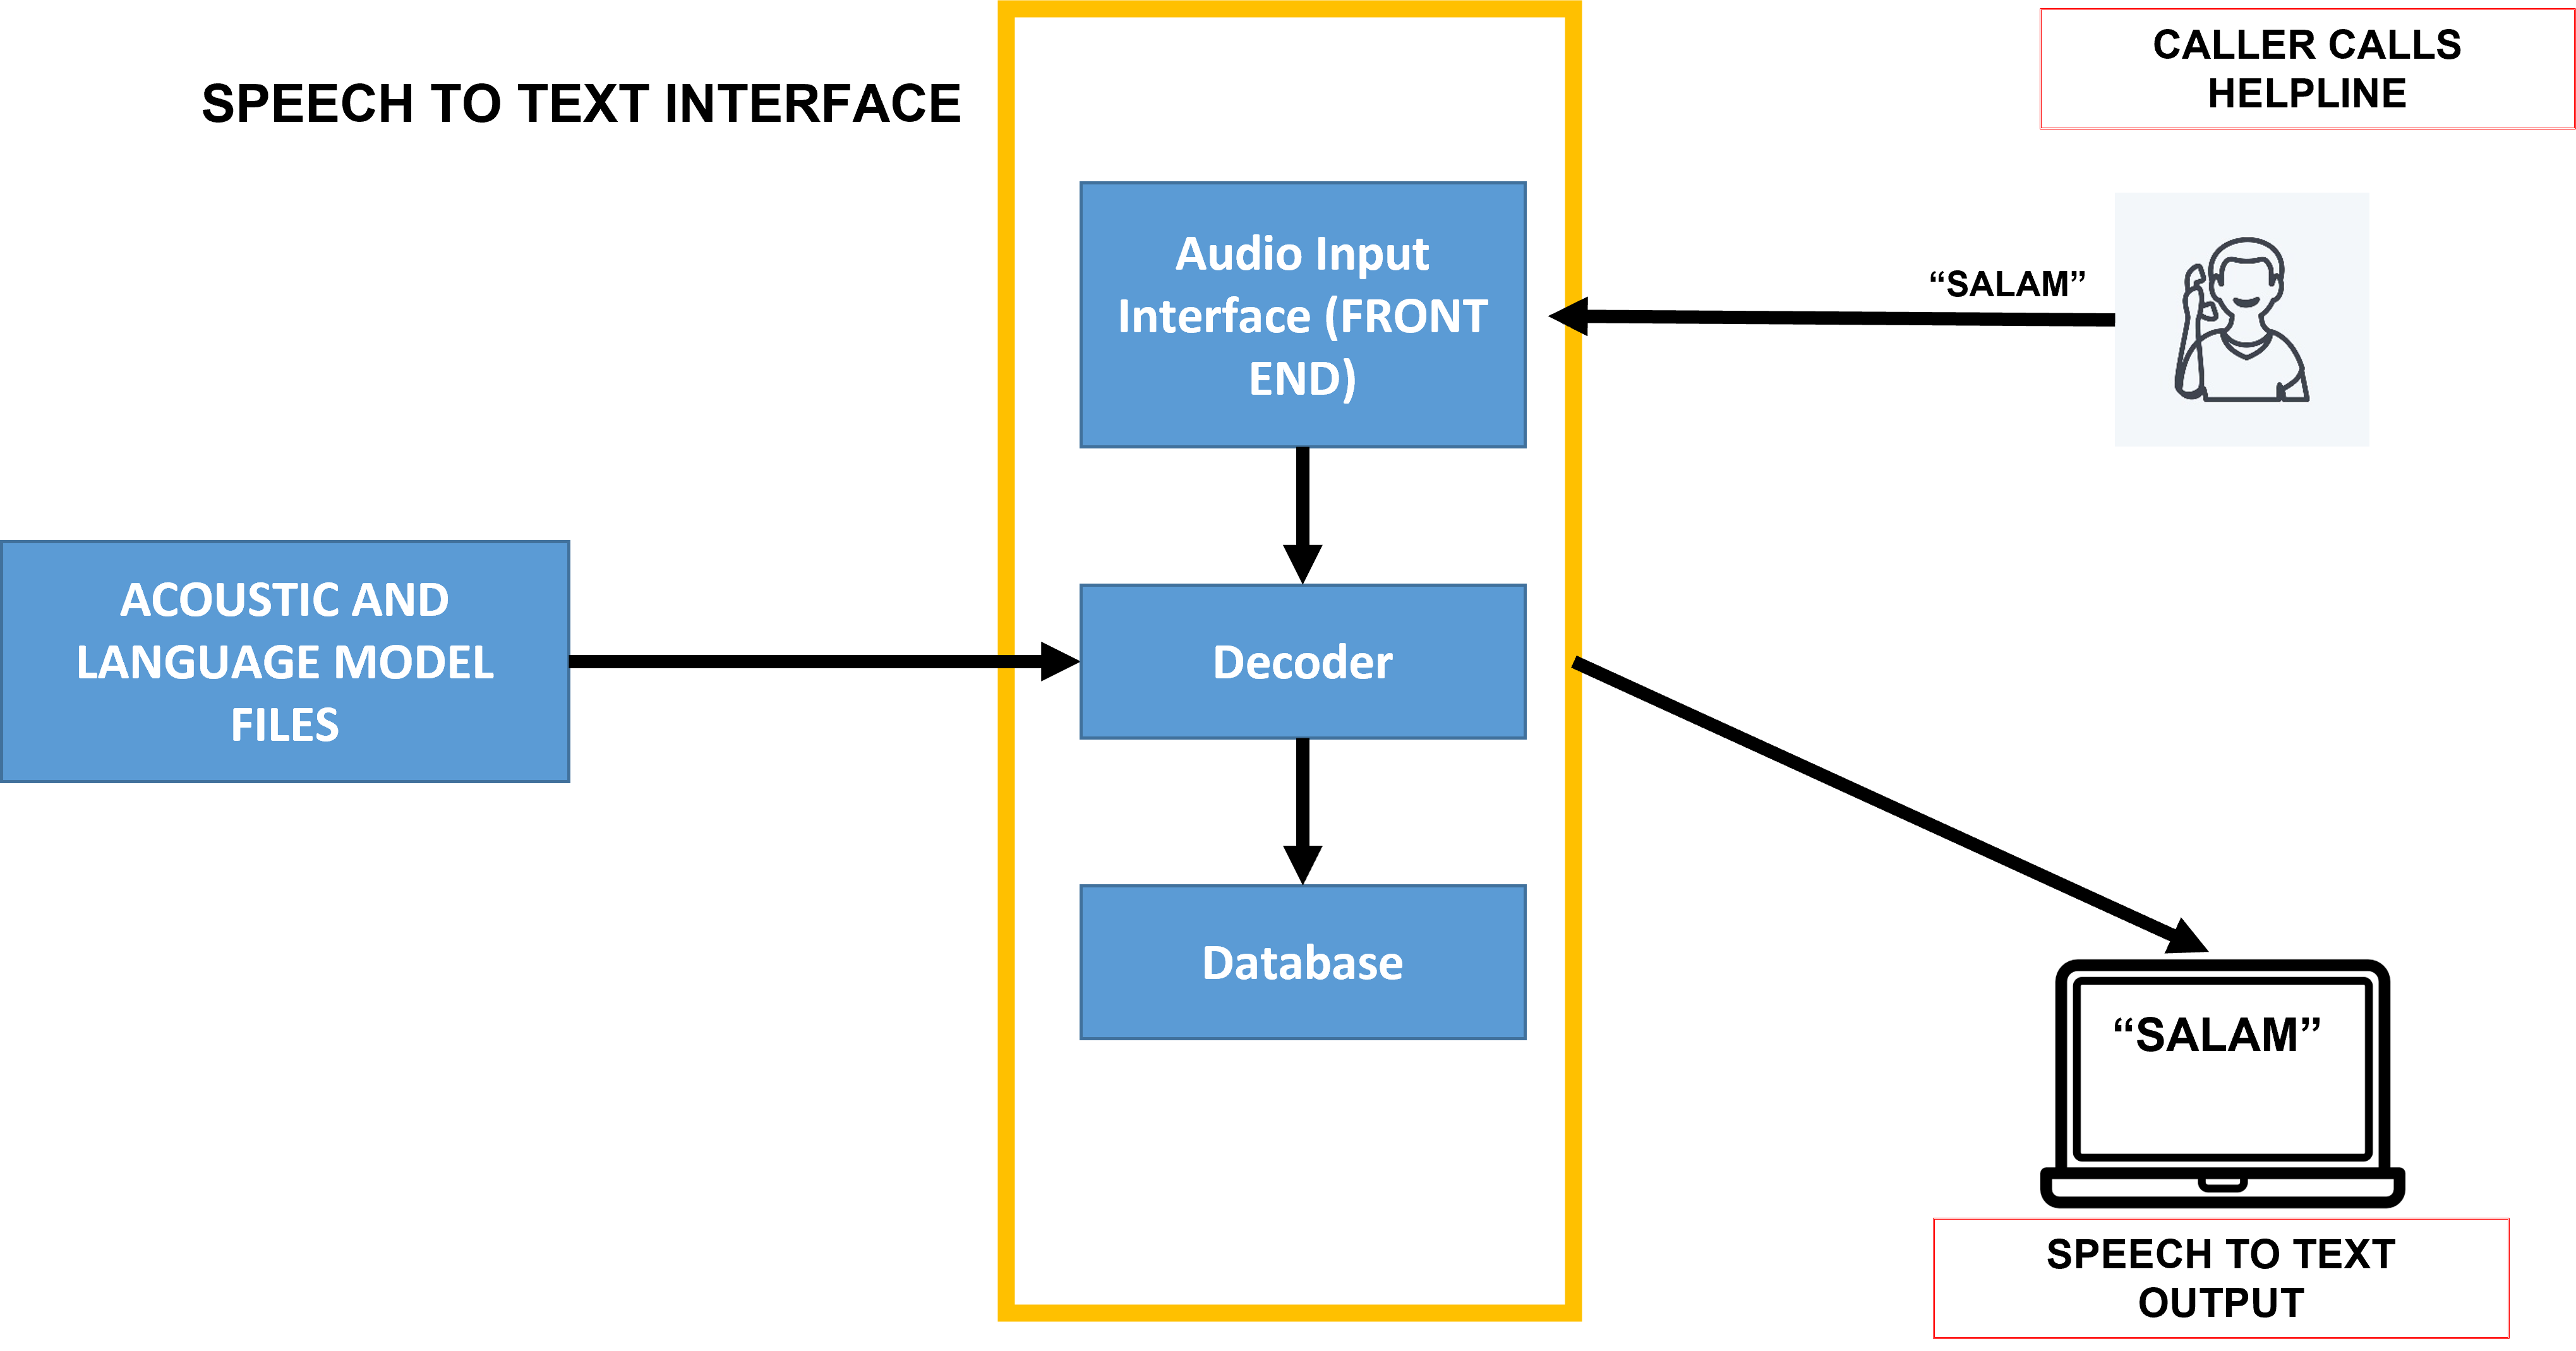
\includegraphics[width=0.9\textwidth]{img/STT2.png}
    \caption{The Speech To Text Interface allows us to take audio input (live or recorded) and it uses the trained model files to give us the text transcription of the audio as output.}
    \label{fig:STT-working}
\end{figure}   

%\begin{figure}[htb]
%    \centering
%    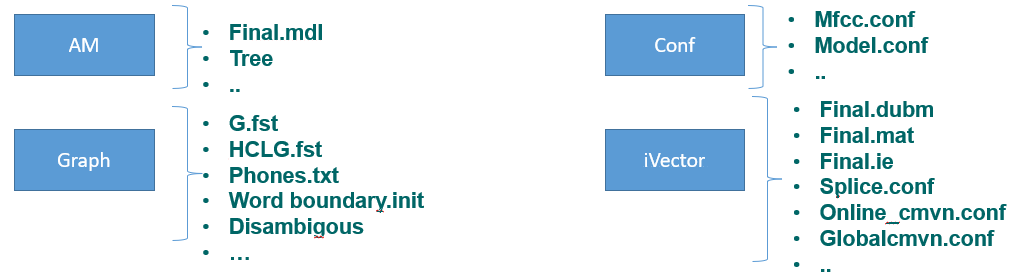
\includegraphics[width=0.7\textwidth]{img/vosk-lm.png}
%    \caption{Model Directory Structure for Speech To Text Interface}
%    \label{fig:vosk-directory-structure}
%\end{figure}    

ASR engines produce very huge model files which add to computational load, storage problems and cross platform deployment issues. We needed an interface that utilizes the necessary language and acoustic model files and provides Speech To Text services on audio signals (live or recorded),  reducing size of the model making it portable and cross-platform compatible. 

We used an offline speech recognition library that comes with a set of accurate models, scripts, and practices and provides ready-to-use speech recognition for different platforms like mobile applications or Raspberry Pi since the model size reduced from 1-5GB to 50-500MB. We can also use this Platform to build a life-long learning platform \cite{eeckt_continual_2021} which continuously improves speech recognition for major languages and use cases \cite{alphacep_vosk_2022}.
